% GRUNDEINSTELLUNGEN -------------------------------------------

\documentclass[a4paper]{article}
\usepackage[ngerman]{babel}
\usepackage[utf8]{inputenc}


% EINGEBUNDENE PAKETE ------------------------------------------

\usepackage{pdfpages} % andere PDFs einbinden
\usepackage{verbatim} % program listings
\usepackage{latexsym} % Symbole zB Box
\usepackage{amssymb} % z.B. mathbb{}
\usepackage{amsmath} 
\usepackage{amsthm} % Für Lemmata, Sätze(Theoreme), Beweise (siehe unten)
\usepackage{tikz}	% Für Diagramme aus dem Programm Dia
\usepackage{makeidx} % fuer Stichwortverzeichnis
\usepackage{csquotes}

% Verweise anklickbar machen
\usepackage{hyperref} % 1. 
\usepackage[figure]{hypcap} % 2. 


% EIGENE BEFEHLE -----------------------------------------------

% Bildbreite: Originalgröße oder falls größer als Seitenbreite/Spalte ==> skalieren
\makeatletter
\def\ScaleIfNeeded{%
\ifdim\Gin@nat@width>\linewidth
\linewidth
\else
\Gin@nat@width
\fi
}
\makeatother

% Neuer Befehl der Bilder standartisiert einbindet:
% includegraphicsdeluxe benötigt \ScaleIfNeeded und \ldate
% 1. innerhalb der figure-Umgebung mit dem Versuch, das Bild mittels [!htb] an genau dieser Position einzufügen
% 2. mit der Original- oder einer skalierten (mittels ScaleIfNeeded s.o.) Größe
% 3. mit einer Beschriftung (\caption{})
% 4. mit einem Label (\label{})
\newcommand{\includegraphicsdeluxe}[3]{
	\begin{figure}[!htb] 
	\centering
	\includegraphics[width=1\ScaleIfNeeded]{pics/\ldate_#1}
	\caption{#2}
	\label{#3}
	\end{figure}
}

% AND und OR Symbole
\newcommand{\und}{\wedge}
\newcommand{\oder}{\vee}

% Grundmengen
\newcommand{\N}{\mathbb{N}}
\newcommand{\Z}{\mathbb{Z}}
\newcommand{\Q}{\mathbb{Q}}
\newcommand{\R}{\mathbb{R}}
\newcommand{\C}{\mathbb{C}}

% Betragsstriche
\newcommand{\abs}[1]{\ensuremath{\left\vert#1\right\vert}}
% Datum der einzelnen Lektionen definieren
\newcommand{\ldate}{2015-05-01}	% define lessiondate
% Anmerkung Professor
\newcommand{\profnote}[1]{\marginpar{\tiny{\textquote{#1}}}}

% Dokumenteneigenschaften
\newcommand{\pTitle}{Diskrete Mathematik}
\newcommand{\pShortName}{M. Zell}
\newcommand{\pSemester}{SS 2015}
\newcommand{\pProfessor}{Prof. Dr. Josef Hörwick}

% EINRÜCKUNG ---------------------------------------------------
\setlength{\parindent}{0pt} % Erste Zeile in Absätzen nicht einrücken.

% KOPF- UND FUSSZEILE ------------------------------------------
\usepackage{fancyhdr}
\pagestyle{fancy}
\fancyhf{}
 
%Kopfzeile mittig mit Kaptilname
\fancyhead[L]{\textsf{\nouppercase{\leftmark}}}
\fancyhead[R]{\textsf{\thepage}}
%Linie oben
\renewcommand{\headrulewidth}{0.5pt}
%Fußzeile 
\fancyfoot[L]{\tiny{\pTitle}}
\fancyfoot[R]{\tiny{\pShortName, \pSemester, \ldate}}
%Linie unten
\renewcommand{\footrulewidth}{0.5pt}
 
% START DES EIGENTLICHEN DOKUMENTS -----------------------------
\author{\pShortName}
\title{Mitschrift\\\pTitle, \pSemester\\\pProfessor}

% Stichwortverzeichnis erstellen
\makeindex

\begin{document}
\maketitle
\newpage
\tableofcontents
\newpage
\listoffigures

% Sätze usw. aus asmthm
\newtheorem{satz}{Satz}[section] 
\newtheorem{defi}{Definition}[section] 
\newtheorem{lem}{Lemma}[section] 
\newtheorem{beh}{Behauptung}[section] 


% einzelne Kapitel
\renewcommand{\ldate}{2015-10-01}

\section{Hinweise}
Diese Mitschrift basiert auf der Vorlesung \textquote{\pTitle} von \pProfessor \ im \pSemester. Du kannst sie gerne benutzen, kopieren und an andere weitergeben. Auch in der Prüfung - soweit zugelassen \footnote{\url{http://www.cs.hm.edu/meinstudium/studierenden_services/fi_pruefungskatalog.de.html}} - kannst du sie gerne als Hilfsmittel verwenden, wenn das meine Nutzung als Prüfungshilfsmittel nicht in irgendeiner Weise beeinträchtigt.\\

Natürlich besteht kein Anspruch auf Aktualität, Richtigkeit, Fortsetzung meines Angebots oder dergleichen. Sollten dir Fehler auffallen oder solltest du Verbesserungsvorschläge haben, würde ich mich über eine E-Mail (zell@hm.edu) freuen. Wenn du mir als kleines Dankeschön z.B. ein Club-Mate\footnote{\url{http://www.clubmate.de/ueber-club-mate.html}} ausgeben möchtest, findest du mich meistens hier: \url{http://fi.cs.hm.edu/fi/rest/public/timetable/group/if3b}. Wenn nicht, ist es auch ok ;-)\\

Nach der Prüfung werde ich den \LaTeX-Quelltext veröffentlichen, damit die Mitschrift weitergeführt, korrigiert und ergänzt werden kann.\\

Viele Grüße\\
\pShortName
% Vorlesung vom 16.03.2015
\renewcommand{\ldate}{2015-03-16}	% define lessiondate

\section{Mengen} 
Mengen\index{Mengen} sind \textbf{ungeordnet} und enthalten \textbf{verschiedene Elemente}: $M=\{4,3,5\}=\{5,4,3\}=\{3,3,4,5\}$. 

\subsection{Mengengleichheit}\index{Mengen!Gleichheit}
Zwei Mengen A und B sind \textbf{gleich}, wenn sie dieselben Elemente enthalten: $x \in A \Leftrightarrow x \in B$.

\subsection{Leere Menge}\index{Mengen!leere} 
Man bezeichnet damit die Menge, die keinerlei Elemente enthält. Die Zeichen für die leere Menge sind $\emptyset$ oder $\{\}$. Die leere Menge ist Teilmenge jeder Menge ($\emptyset \subseteq A$).

\subsection{Unendliche Mengen}\index{Mengen!Unendliche}
Ein Beispiel für unendliche Mengen ist die Menge der natürlichen Zahlen ($\N=\{1,2,3,4,...\}$). Aber auch $M=\{n \in \N : 7 \textrm{ teilt }n\}=\{7,14,21,28,...\}=7 \cdot  \N$

\subsection{Definitionen}

\subsubsection{Teilmenge}\index{Mengen!Teilmenge}
Eine Menge A heißt Teilmenge einer Menge B, wenn jedes Element von A auch Element von B ist. Formal: $A\subset B\ :\Longleftrightarrow \forall x \left(x \in A \,\rightarrow x \in B \right)$.\\
\textbf{Beispiel:} $B=\{2,3,4,5\}, A=\{3,4\}, A\subset B, \emptyset \in B$ \includegraphicsdeluxe{teilmenge_wikipedia.png}{A ist eine (echte) Teilmenge von B}{fig:teilmenge_wikipedia} % Nr. 

\subsubsection{Durchschnitt}\index{Mengen!Durchschnitt}
$A\cap B : \{x : x \in A \und x\in B \}$\\
\textbf{Beispiel:} $A=\{3,5,6\}, B=\{3,\{5,6\},6,7\}, A\nsubseteq B \Rightarrow A\cap B=\{3,6\}$. Bei mehreren Mengen: $\bigcap_{i\in \N} A_i=A_1\cap A_2\cap A_3\cap ... = \{x : \forall i \in \N:x\in A_i\}$
\includegraphicsdeluxe{schnittmenge_wikipedia.png}{Schnittmenge von A und B}{fig:schnittmenge_wikipedia} % Nr. 

\subsubsection{Vereinigung}\index{Mengen!Vereinigung}
$A\cup B : \{x : x \in A \oder x\in B \}$\\
\textbf{Beispiel:} $A=\{3,5,6\}, B=\{3,\{5,6\},6,7\}, A\nsubseteq B \Rightarrow A\cup B=\{3,5,6,7,\{5,6\}\}$. Bei mehreren Mengen: $\bigcup_{i\in \N} A_i=A_1\cup A_2\cup A_3\cup ... = \{x : \exists i : x\in A_i\}$, auch: $\bigcup_{i=1}^3 A_i=A_1 \cup A_2 \cup A_3$
\includegraphicsdeluxe{vereinigungsmenge_wikipedia.png}{Vereinigungsmenge von A und B}{fig:vereinigungsmenge_wikipedia} % Nr. 

\subsubsection{Differenz}\index{Mengen!Differenz}
$A \setminus B := \{ x \mid \left( x\in A \right) \und \left( x\not\in B \right) \}$\\
\textbf{Beispiel:} $B\setminus A=\{\{5,6\},7\}$
\includegraphicsdeluxe{differenz_wikipedia.png}{B ohne A}{fig:differenz_wikipedia} % Nr. 

\subsubsection{Grundmenge $ \Omega $ }\index{Mengen!Grundmenge}
$A \subset \Omega \rightarrow \bar A=\Omega \setminus A$, auch: $\bar A=\{x \in \Omega:x\notin A\}$

\begin{satz}
$A=B \Leftrightarrow A\subset B \und B\subset A$
\end{satz}

\begin{satz}
Es gilt:
\begin{itemize}
\item $\overline{\bigcup_{i\in \N}A_i}=\bigcap_{i\in \N} \overline{A_i}$
\item $\overline{\bigcap_{i\in \N}A_i}=\bigcup_{i\in \N} \overline{A_i}$
\end{itemize}
\end{satz}

\begin{proof}
Sei
\begin{itemize}
\item $x\in \overline{\bigcup_{i\in \N}A_i} \Leftrightarrow x\notin \bigcup_{i\in \N} A_i \Leftrightarrow x\notin A_i \forall i \in \N \Leftrightarrow x\in \overline{A_i} \forall i\in \N \Leftrightarrow x\in \bigcap_{i\in \N} \overline{A_i}$ 
\item  $x\in \overline{\bigcap_{i\in \N} A_i} \Leftrightarrow x\notin \bigcap_{i\in \N} A_i \Leftrightarrow \exists i \in \N \textrm{ mit } x\notin A_i \Leftrightarrow \exists i \in \N \textrm{ mit }x\in \overline{A_i} \Leftrightarrow x\in \bigcup_{i\in \N} \overline{A_i}$
\end{itemize}
\end{proof}

\subsection{Potenzmenge}\index{Mengen!Potenzmenge}
Die Potenzmenge P(M) ist die Menge aller Teilmengen von M. Beispiel: $M=\{1,2,3\} \Rightarrow P(M)=\{\{1\},\{2\},\{3\},\{1,2\},\{1,3\},\{2,3\},\{1,2,3\},\{\}\}$. Es fällt auf, dass P(M) 8 Elemente also die Mächtigkeit $|P(M)|=8=2^3$ hat. 

\subsubsection{Mächtigkeit von Mengen}\index{Mengen!Mächtigkeit}\index{Mengen!Kardinalität} Die Mächtigkeit von Mengen heißt auch Kardinalität. 

\begin{satz}
Sei M endlich: $|P(M)|=2^{|M|}$
\end{satz}

\begin{proof}
Jede Abbildung $f:M \longmapsto {0,1}$ entspricht einer Teilmenge A von M. $x\in A \Leftrightarrow f(x)=1$. Wir zählen die Abbildungen $f:M \longmapsto {0,1}$:\\
$M=
\begin{array}{ccccc}
1 & 2 & 3 & 4 & 5 \\ 
\downarrow & \downarrow & \downarrow & \downarrow & \downarrow \\ 
0 & 1 & 1 & 0 & 1 \\ 
\end{array} 
\Rightarrow 2 \cdot  2 \cdot  2 \cdot  2 \cdot  2 = 2^5
$ Möglichkeiten für f.
\end{proof}

\section{Relationen}\index{Relationen}

\subsection{Das Direkte Produkt von zwei Mengen}\index{Relationen!Direktes Produkt}
$A\times B=\{(a,b):a\in A,b\in B\}$\\
Es gilt: $(a,b)=(c,d) \Leftrightarrow a=c \textrm{ und } b=d$\\
\paragraph{Beispiel:} $A=\{1,2,3\}, B={a,b} \Rightarrow A\times B=\{(1,a),(2,a),(3,a),(1,b),(2,b),(3,b)\}$

\subsection{Relation}
Eine Relation R auf A,B ist eine Teilmenge von $A\times B$, z.B.: $A=\{1,2,3\}, B=\{a,b\}, R=\{(1,a),(2,b),(3,b)\}$. Für $(1.a)\in \R$ schreibt man auch 1 R a oder 1 $\sim$ a.\marginpar{Für Relationen kann man beliebige Zeichen verwenden, hier eben $\sim$.} Die beiden Mengen A,B können gleich sein. Relationen auf A,A oder kurz: Relation auf A: $A=\{1,2,3\}, R=\{(1,2),(1,3),(2,3)\}$ oder 

\paragraph{Beispiel:}Relation auf $\N$: $A=\N$\\
$\leq:\{(a,b)\in \N^2:a\leq b\}$\\
$=:\{(a,b)\in \N^2:a=b\}=\{(a,a):a\in \N \}$\\

\subsection{Äquivalenzrelation}\index{Relationen!Äquivalenzrelation}
Sei v eine Relation auf M mit folgenden Eigenschaften: 
\begin{enumerate}
\item $a\sim a, \forall a\in M$ (reflexiv)\index{Relationen!reflexiv}
\item $a\sim b \Rightarrow b\sim a$ (symmetrisch)\index{Relationen!symmetrisch}
\item $a\sim b \und b\sim c \Rightarrow a\sim c$ (transitiv)\index{Relationen!transitiv}
\end{enumerate}

\paragraph{Beispiel:}$M=$ist die Menge von Kugeln mit den Farben rot, blau, weiß. Kugel a $\sim$ Kugel b $\Leftrightarrow a,b$ haben dieselbe Farbe:
\begin{itemize}
\item $\sim$ ist reflexiv $\checkmark$
\item $\sim$ ist symmetrisch $\checkmark$
\item $\sim$ ist transitiv $\checkmark$
\end{itemize}
$\Rightarrow\ \sim$ ist Äquivalenzrelation.

\subsection{Grundmenge $\Z$}
$x\sim y \Leftrightarrow x-y\in 5\cdot \Z=\{5z:z\in\Z\}=\{-10,-5,0,5,10,...\}$\\
$x\sim y \Leftrightarrow x \textrm{ und } y$ unterscheiden sich durch ein Vielfaches von 5, z.B.: $3\sim 8, -7\sim 3, -8\sim -23$. 
\begin{itemize}
\item $\sim$ ist reflexiv $\checkmark$
\item $\sim$ ist symmetrisch $\checkmark$
\item $\sim$ ist transitiv $\checkmark$
\end{itemize}
$\Rightarrow\ \sim$ ist Äquivalenzrelation.

\begin{defi}[Äquivalenzklassen]\index{Relationen!Äquivalenzklassen}
$\sim$ sei eine Äquivalenzrelation auf M, dann gilt:\\
$[x]=\{y\in M: x\sim y\}$ heißt Äquivalenzklasse von x. Natürlich gilt auch: $x\in[x]$.
\end{defi}

\begin{satz}
Die Äquivalenzklassen bilden eine Zerlegung von M. 
\end{satz}
\includegraphicsdeluxe{aequivalenzklassen_wikipedia.png}{Menge von acht Buchexemplaren mit eingezeichneter Äquivalenzrelation „x und y besitzen dieselbe ISBN“ als Pfeildiagramm und den Äquivalenzklassen (Quelle: Wikipedia).}{fig:aequivalenzklassen_wikipedia} % Nr. 
\begin{proof}
Falls $y\in [x]$, so ist $[y]=[y]$\\
$\left.
\begin{array}{c}
\textrm{Sei } a\in [x] \Rightarrow a\sim x \Rightarrow a\sim y \Rightarrow a\in [y] \Rightarrow [x]\subset [y] \\ 
\textrm{Sei } a\in [y] \Rightarrow a\sim y \Rightarrow a\sim x \Rightarrow a\in [x] \Rightarrow [y] \subset [x]
\end{array} 
\right\}[x]=[y]$\\
Falls $[x] \cap [y] \neq \emptyset$, z.B.: $a\in [x]$ und $a\in [y] \Rightarrow [a]=[x]=[y]$, also $[x]=[y] \Rightarrow$ Zerlegung von M. 
\end{proof}

\paragraph{Beispiel:} Die Zerlegung durch die Äquivalenzklassen kann man anhand des Beispiels $x\sim y \Leftrightarrow x-y\in 5\cdot \Z$ gut auf einem Zahlenstrahl zeigen (Abb. \ref{fig:aequivalenzklassen_auf_zahlenstrahl}).

\noindent blau: $\overbrace{[0]}^{\textrm{Klassen}}=\overbrace{\{...,-10,-5,0,5,10,...\}}^{\textrm{Jeder Wert kann Representant der Klasse sein}}=[15]=[-5]$\\
rot: $[1]=\{...,-9,-4,1,6,...\}=[6]=[-4]$\\
grün: $[2]=\{...,-8,-3,2,7,...\}=[-8]=[7]$\\ 

%\includegraphicsdeluxe{aequivalenzklassen_auf_zahlenstrahl.jpg}{Zerlegung von $\Z$ in 5 Klassen}{fig:aequivalenzklassen_auf_zahlenstrahl} % Nr. 2
Die Zerlegung einer Menge M in Klassen entsprechn den Äquivalenzrelationen auf M.

\subsection{Funktionen}\index{Funktionen}

\begin{defi}[Funktion]
Eine Relation R auf den Mengen A,B heißt Funktion von A nach B, wenn gilt: Zu jedem $a\in A$ gibt es genau ein $b\in B$ mit $(a,b)\in R$.
\end{defi}

\paragraph{Schreibweise:}
$f: 
\begin{cases} 
A \rightarrow B \\
a \rightarrow f(a)
\end{cases}$\\
mit A Definitionsbereich\index{Funktionen!Definitionsbereich}, B Zielbereich\index{Funktionen!Zielbereich}, R Graph\index{Funktionen!Graph} von A ($R=\{(a,f(a)):a\in A\}$) und W Wertebereich\index{Funktionen!Wertebereich} ($\{f(a):a\in A\}$).

\begin{defi}[Bild von D]\index{Funktionen!Bild}
Sei $D\subset A: f(D)=\{f(x):x\in D\}$ (auch: Zielmenge, Wertemenge, Wertebereich)
\end{defi}

\begin{defi}[Urbild von E]\index{Funktionen!Urbild}
Sei $E\subset B: f^{-1}(E)=\{x\in A: f(x)\in E\}$.
Das Urbild einer Teilmenge der Zielmenge von f ist eine Teilmenge der Definitionsmenge.
\end{defi}

\begin{defi}[injektiv, auch: linkseindeutig]\index{Funktionen!injektiv}
Sei $f:A\rightarrow B$. f ist injektiv, falls $x,y\in A$ und $x\neq y \Rightarrow f(x)\neq f(y)$
\end{defi}
%\includegraphicsdeluxe{fnk_injektiv.jpg}{Elemente in B werden einmal oder gar nicht getroffen}{fig:fnk_injektiv} % Nr. 3
Elemente aus A bilden nicht auf dasselbe Element in B ab. Wie kann man zeigen, dass eine Funktion injektiv ist? Zeige: $f(x)=f(y) \Rightarrow x=y$.

\begin{defi}[surjektiv, auch: rechtstotal]\index{Funktionen!surjektiv}
Sei $f:A\rightarrow B$. f ist surjektiv, falls $f(a)=B$
\end{defi}
%\includegraphicsdeluxe{fnk_surjektiv.jpg}{Jedes Element der Zielmenge B wird mindestens einmal als Funktionswert angenommen.}{fig:fnk_surjektiv} % Nr. 4
Auf jedes Element der Wertemenge B wird abgebildet.  

\begin{defi}[bijektiv]\index{Funktionen!bijektiv}
Sei $f:A\rightarrow B$. f ist bijektiv, wenn injektiv und surjektiv.
\end{defi}
%\includegraphicsdeluxe{fnk_bijektiv.jpg}{}{fig:fnk_bijektiv} % Nr. 5
f bijektiv, dann immer umkehrbar. Man kann die Umkehrfunktion definieren: $f^{-1}:B\rightarrow A, b\rightarrow a$ mit $f(a)=b$
\begin{proof}Sei $f:A\rightarrow B$\\
f surjektiv $\Rightarrow \exists a$ mit $f(a)=b$\\
f injektiv $\Rightarrow$ Es gibt höchstens ein a mit f(a)=b.
\end{proof}

\subsubsection{Umkehrabbildung}\index{Funktionen!Umkehrabbildung}\index{Funktionen!Umkehrfunktion}
$f:
\begin{array}{ccc}
1 & 2 & 3 \\ 
\downarrow & \downarrow & \downarrow \\ 
5 & 0 & 3
\end{array} 
$
\\
$f^{-1}:
\begin{array}{ccc}
0 & 3 & 5 \\ 
\downarrow & \downarrow & \downarrow \\ 
2 & 3 & 1
\end{array} 
$
\\
Die Umkehrfunktion von $f^{-1}$ ist f.

\subsubsection{Komposition}
\begin{defi}[Komposition]\index{Funktionen!Komposition}
Für A $\xrightarrow{f}$ B $\xrightarrow{g}$ C schreibt man auch $g \circ f$ (Komposition): $g\circ f: A\rightarrow C,a\rightarrow g(f(a))$\\
Es seien f und g ein Paar von Funktion und Umkehrfunktion.\\
$(g\circ f)(x)=x, g\circ f=id$\\
$(f\circ g)(x)=x, f\circ g=id$\\
$id(x)=x$\\
\end{defi}

\begin{satz}
$f:A\rightarrow B$ ist injektiv\index{Funktionen!injektiv} $\Rightarrow \exists g:B\rightarrow A$ mit $g\circ f=id$. 
\end{satz}

% ausgelassen: Beweis


% Vorlesung vom 11.05.2015
\renewcommand{\ldate}{2015-05-11}	% define lessiondate

\section{Fehlererkennung}

\subsection{Fehlererkennender Code}
Teilmenge C von V. Sender schickt $ c \in C$. Empfänger empfängt c' aus V. Ist c' in C akzeptiert er, sonst lehnt er ab.
\paragraph{Beispiel (Übermitteln einer Vierstellige Zahl ):} Man fügt eine fünfte Zahl (Kontrollzahl) hinzu, sodass die $ Quersumme = 0 \ \mbox{mod} \ 10 $ ist. \marginpar{\textit{Es soll ein Vielfaches von 10 rauskommen}}\\
$ V=\{(a_1,...,a_5) : a_i = 0,1,...,9\} $\\
$ C=\{(a_1,...,a_5) \in V: a_1 + a_2 + a_3 + a_4 + a_5 = 0 \ \mbox{mod} \ 10\} $\\
\textbf{Code n zur Basis q:} $ C=\{(a_1,...,a_5) : 0 \leq a_i \leq q-1\} $\\
\textbf{Paritätscode:} Code der Länge n zur Basis q und 
\[ C \equiv \{(a_1,...,a_5) : 0 \le a_1 \le q-1 \ \mbox{und} \ a_1 + ... + a_n = 0 \equiv q \}\]

\paragraph{Beispiel:} $n=5, q=11$. Ist der Code $ (3,0,10,4,5) \in C$?\\
$ 3+0+10+4+5=22 $

\paragraph{Satz} 
Jeder Paritätscode erkennt Einzelfehler (eine Stelle ändern). 

\paragraph{Beweis}
Das Codewort ist $a_1,...,a_i,...,a_n $ Codewort\\
Es kommt zu einem Fehler $a_1,...,\underbrace{a_i'}_{Fehler},...,a_n \ $\\
\[a_1 + a_i' + ... + a_n - \underbrace{(a_1 + ... + a_i + ... + a_n)}_{0} = 
a_i' - a_i \neq 0 \ \mbox{mod} \ q\]\\
\textbf{Vertauschungsfehler:} $a_i$ und $a_j$ werden vertauscht. Ein Paritätscode erkennt keinen Vertauschungsfehler!

\paragraph{Idee: Gewichte!} Basis q, n Stellen, Gewichte $g_i \ \mbox{mit} \ 1 \le g_i \le q-1$ \\
$ g_1 a_1 + ... + g_n a_n \equiv 0 \ \mbox{mod} \ q$ 

\paragraph{Satz:}
Ist $g_n$ teilerfremd zu q, so kann man immer die Kontrollziffer $a_n$ ausrechnen.

\paragraph{Beweis}
$ g_1 a_1 + ... + g_n a_n = 0$ \marginpar{mod $q$ !}\\ 
$ g_n a_n = - g_1 a_1 - ... - g_{n-1} a_{n-1}$\\
\[a_n = \underbrace{g_{n}^{-1}}_{\mbox{existiert, da } g_n \ \mbox{teilerfremd zu } q.} (- g_1 a_1 - ... - g_{n-1} a_{n-1})
\]


\paragraph{Satz:} Ein Paritätscode mit Gewichten erkennt jeden Einzelfehler der Stelle $a_i$, wenn $g_i$ und $q$ teilerfremd sind.

\paragraph{Beweis:} 
$a_1 \rightarrow a_1' (falsch)$\\
$g_1 a_1' + ... + g_n a_n = $\\
$g_1 a_1' + ... + g_n a_n - (g_1 a_1 + ... + g_n a_n) = $\\
$g_1 a_1' - g_1 a_1 = \underbrace{\underbrace{g_1}_{\neq 0} \underbrace{(a_1' - a_1)}_{\neq 0}}_{\mbox{Einheit (} g_1 \ \mbox{teilerfremd zu }q \ \mbox{). Kein Nullteiler.}} \neq 0$\\

\paragraph{Folgerung:} Damit man alle Einzelfehler erkennen kann, müssen $g_i$ teilerfremd zu $q$ sein.

\paragraph{Satz:} Ein Paritätscode mit Gewichten erkennt den Vertauschungsfehler $a_i \leftrightarrow a_j$, wenn $g_i - g_j$ teilerfremd zu q ist. 

\paragraph{Beweis:} Vertauschungsfehler, z.B.: $ a_1 \leftrightarrow a_2$\\
$g_1 a_2 + g_2 a_1 + g_3 a_3 + ... + g_n a_n =$\\
$g_1 a_2 + g_2 a_1 + ... + g_n a_n - (g_1 a_1 + ... + g_n a_n) =$\\
$g_1 a_2 + g_2 a_1 - g_1 a_1 - g_2 a_2 =$\\
$g_1(a_2 - a_1) + g_2(a_1 - a_2) =$\\
$g_1(a_2 - a_1) - g_2(a_2 - a_1) =$\\
$\underbrace{\underbrace{(g_1 - g_2)}_{\neq 0} \underbrace{(a_2-a_1)}_{\neq 0}}_{Einheit, kein Nullteiler} \neq 0$\marginpar{mod q}\\


\paragraph{Beispiel:} Ein Paritätscode der Länge 10 zur Basis $q=11$.\\ 

\begin{tabular}{ccccccccccc}
 & $a_1$ & $a_2$ & $a_3$ & $a_4$ & $a_5$ & $a_6 $ & $a_7 $ & $a_8 $ & $a_9 $ & $a_{10}$\\ 
$g_i$ & 10 & 9 & 8 & 7 & 6 & 5 & 4 & 3 & 2 & 1\\ 
\end{tabular} 
Erkennt jeden Einzelfehler und jeden Vertauschungsfehler! Das ist der ISBN-Code bei den Büchern (10=X).

\paragraph{Beispiel (ISBN-Code):} "Die letzte Stelle \textbf{2} kann nicht einfach gewählt werden, sondern muss stimmen! "\\
\begin{tabular}{c|cccccccccc}
 & $a_1$ & $a_2$ & $a_3$ & $a_4$ & $a_5$ & $a_6 $ & $a_7 $ & $a_8 $ & $a_9 $ & $a_{10}$\\ \hline
 & 3 & 1 & 5 & 7 & 2 & 2 & 1 & 8 & 9 & \textbf{2}\\
$g_i$ & 10 & 9 & 8 & 7 & 6 & 5 & 4 & 3 & 2 & 1\\ 
Produkt 30 & 9 & 40 & 49 & 12 & 10 & 4 & 24 & 18 & \\
mod 11 & 8 & 9 & 7 & 5 & 1 & 10 & 4 & 2 & 7 & \textbf{2}\\
\end{tabular} 
\marginpar{$\sum=8+9+7+5+1+10+4+2+7=53=9$} 

\subsection{Codes über Gruppen}
\paragraph{Wiederholung:}
$(G,\cdot)$ ist eine Gruppe, wenn:
\begin{itemize}
\item $\cdot$ ist assoziativ
\item Es gibt ein neutrales Element e
\item Jedes a hat ein Inverses b, d.h. $ab=ba=e$
\end{itemize}
Das Inverse ist eindeutig und heißt $a^{-1}$

\paragraph{Satz}
Gleichungen der Form $ax = b$ sind eindeutig lösbar.

\paragraph{Beweis:}
\begin{itemize}
\item Sei x eine Lösung $\Rightarrow a x = b \Rightarrow x = a^{-1} b$
\item Setze $x = a^{-1} b \Rightarrow a a^{-1} b = b$
\end{itemize}
$\Box$

\paragraph{Satz:} 
Die Abbildung 
\begin{equation*}
 a_l:\qquad	
 \left\{
 \begin{aligned}
	G \rightarrow G\\
	x \rightarrow ax
	\end{aligned}
	\right.
\end{equation*}
ist bijektiv. 

\paragraph{Beweis:}
\begin{itemize}
\item injektiv: Sei $ax=ay \Rightarrow x=y$
\item surjektiv: Falls $\vert G \vert$ endlich (klar!), $ax = b; x = a^{-1} b$
\end{itemize}
$\Box$

\paragraph{Beispiel 1:}
$(\mathbb{Z},+), (\mathbb{Z}_n,+)$, $(\mathbb{Z}_n^* ,\cdot), (\mathbb{R},+), (\mathbb{R}^* ,\cdot)$ Gruppen

\paragraph{Beispiel 2:}
Menge M: $G = \{f \colon M \rightarrow M, \mbox{mit f bijektiv}\}$ \\
Komposition: (Hintereinanderausführung) $(G,\cdot) \ \mbox{Gruppe.} \ e=id$  $id(x)=x$. Das Inverse von f ist die Umkehrabbildung $f^{-1}$

\paragraph{Beispiel 3:}
Eine bijektive Abbildung der Ebene in sich heißt \underline{Kongruenz}, wenn sie die Abstände erhält: $ d(x,y) = d(\varphi(x), \varphi(y)) \Rightarrow$ Winkel bleiben erhalten. \\
Die Kongruenzen (vgl. Abb. \ref{fig:kongruenzen}) bilden bezüglich $\circ$ eine Gruppe.
\begin{itemize}
\item Verschiebungen
\item Spiegelungen
\item Drehungen
\item Gleitspiegelungen
\end{itemize}


\includegraphicsdeluxe{kongruenzen.jpg}{Das sind alle Kongruenzen}{fig:kongruenzen}

\paragraph{Beispiel 4 (Symmetrie einer ebenen Figur):}
Alle Kongruenzen, welche die Figur auf sich abbilden, bilden eine Gruppe (vgl. Abb. \ref{fig:rechteck}). 


\includegraphicsdeluxe{rechteck.jpg}{Spiegelungen an h,g, Drehungen um Z um 180$^\circ$ und id}{fig:rechteck}


\textbf{Gruppentafel} \marginpar{\textbf{g}: wegen $dr \circ h = g$ (erst h, dann dr)\\ $1 \rightarrow 4$\\ $2 \rightarrow 3$\\ $3 \rightarrow 2$\\ $4 \rightarrow 1$}\\
\begin{tabular}{|c|c|c|c|c|}
\hline $ \circ $ & id & dr & h & g \\ 
\hline id & id & dr & h & g \\ 
\hline dr & dr & id & \textbf{g} & h \\ 
\hline h & h & g & id & dr \\ 
\hline g & g & h & dr & id \\ 
\hline 
\end{tabular}
\\

\paragraph{Definition:} 
Code über Gruppe $(G,\cdot)$ der Länge $n$ und Kontrollsymbol $c \in G$: $\{(a_1,...,a_n) \colon a_i \in G \ \mbox{und} \ a_1 a_2 ... a_n = c\}$

\paragraph{Satz:}Ein Gruppencode erkennt Einzelfehler. 

\paragraph{Beweis:}  
\[
\begin{array}{c}
(1) \ a_1 (a_2 ... a_n) = c\\
(2) \ a_1' (a_2 ... a_n) = c \\
\Rightarrow a_1 = a_1' \Box\\
\end{array}
\]

Ein Gruppencode kann einen Vertauschungsfehler erkennen oder nicht. Ist G kommutativ, so werden Vertauschungsfehler \textbf{nicht} erkannt. \marginpar{Eine Gruppe eignet sich umso besser, je weniger sie kommutativ ist.}\\
$a_1 a_2 (a_3 ... a_n) = c$\\
$a_2 a_1 (a_3 ... a_n) = c$\\
$\Rightarrow a_1 a_2 = a_2 a_1$\\

\subsection{Permutationen}
Eine Permutation ist eine bijektive Abbildung einer endlichen Menge auf sich. 
$ \pi_1:  
\begin{array}{ccccc}
1 & 2 & 3 & 4 & 5 \\ 
 \downarrow  &  \downarrow  &  \downarrow  &  \downarrow  &  \downarrow  \\ 
2 & 3 & 1 & 5 & 4
\end{array} $
\\
$ \pi_2: 
\begin{array}{ccccc}
1 & 2 & 3 & 4 & 5 \\ 
\downarrow & \downarrow & \downarrow & \downarrow & \downarrow \\ 
5 & 1 & 2 & 4 & 3
\end{array} $
\\
$ \pi_1 \circ \pi_2
\begin{array}{ccccc}
1 & 2 & 3 & 4 & 5 \\ 
\downarrow & \downarrow & \downarrow & \downarrow & \downarrow \\ 
1 & 2 & 5 & 3 & 4
\end{array} $
\\
$ \pi_2^{-1} 
\begin{array}{ccccc}
1 & 2 & 3 & 4 & 5 \\ 
\downarrow & \downarrow & \downarrow & \downarrow & \downarrow \\ 
2 & 3 & 5 & 4 & 1
\end{array} $

\paragraph{Gruppencode mit Permutationen:} 
Länge n, Gruppe G, Permutationen der Gruppe: $ \pi_1,  \pi_2, ...,  \pi_n$, Kontrollsymbol $ c \subset G$.\\
$ C = \{(a_1, ..., a_n) \colon a_i \in \ \mbox{G und} \ \pi_1(a_1) \pi_2(a_2) ....  \pi_n(a_n) = c\}$

\paragraph{Satz:}
Ein Gruppencode mit Permutationen erkennt Einzelfehler. 

\paragraph{Beweis:}
$\pi_1(a_1) ....  \pi_n(a_n) = c$\\
$\pi_1(a_1')  \pi_2(a_2) ....  \pi_n(a_n) = c$\\
$\Rightarrow \pi_1(a_1) = \pi_1(a_1') \Rightarrow a_1 = a_1'$\\
$\Box$

\paragraph{Satz:}
Ein Gruppencode mit Permutationen erkennt den Vertauschungsfehler der Stellen $i, i+1$, wenn Folgendes gilt:
\begin{itemize}
\item $\pi_i(g) \cdot  \pi_{i+1}(h) \neq \pi_i(h) \cdot  \pi_{i+1}(g) \ \forall g \neq h$
\end{itemize}
"klar" $\Box$

\paragraph{Beispiel (Code der deutschen Geldscheine):}
Gruppe: \textit{Diedergruppe} Ordnung 10. Das sind die Symmetrien des regelmäßigen 5-Ecks:

\includegraphicsdeluxe{fuenfeck.jpg}{Fünfeck: 5 Spiegelungen, 4 Drehungen, id (10)}{fig:fuenfeck}

Bilden Gruppe (10 Elemente). Wir bezeichnen die Symmetrien mit $0,1,...,9 \ (0 \widehat{=} id)$. Der Code soll die Länge n = 11 haben. Das Kontrollsymbol c sei 0. Wir benötigen 11 Permutationen. 

$ \pi_1:
\begin{array}{cccccccccc}
0 & 1 & 2 & 3 & 4 & 5 & 6 & 7 & 8 & 9 \\ 
\downarrow & \downarrow & \downarrow & \downarrow & \downarrow & \downarrow & \downarrow & \downarrow & \downarrow & \downarrow \\ 
1 & 5 & 7 & 6 & 2 & 8 & 3 & 0 & 9 & 4
\end{array} $
\\
$ \pi_2 = \pi_1 \circ \pi_1 = \pi_1^2 $ \\
$ \pi_3 = \pi_1 \circ \pi_1 \circ \pi_1 = \pi_1^3 $ \\
$ \vdots $ \\
$ \pi_{11} = \pi_1^{11} $ \\
$ Code = \{(a_1,a_2,...,a_{11}) \colon 0 \le a_i \le 9 \ \mbox{und} \ \pi_1(a_1) \pi_2(a_2) ... \pi_{11}(a_{11}) = 0 \} $ \\ 
Wie berechnet man die "Kontrollziffer" $a_{11}$?\marginpar{$c = 0$}\\
$\pi_1(a_1) ... \pi_{11}(a_{11}) = c $\\
$\pi_{11}(a_{11}) = [\pi_1(a_1) ... \pi_{10}(a_{10})]^{-1} \cdot  c$\\
$a_{11}=\pi_{11}^{-1} [(\pi_{1}(a_{1} ... \pi_{10}(a_{10}))^{-1} \cdot  c]$

\paragraph{Beispiel (Symmetrie eines gleichseitigen Dreiecks)}
Spiegelungen w1, w2, w3, Drehungen um Z 120, 240 und id (vgl. Abb. \ref{fig:gleichseitigesDreieck})

\includegraphicsdeluxe{gleichseitiges-dreieck.jpg}{Gleichseitiges Dreieck}{fig:gleichseitigesDreieck}


\textbf{Gruppentafel}\\
\begin{tabular}{|c|c|c|c|c|c|c|}
\hline $\circ$ & id & w1 & w2 & w3 & 120 & 240 \\ 
\hline id & id & w1 & w2 & w3 & 120 & 240 \\ 
\hline w1 & w1 & id & 120 & 240 & w2 & w3 \\ 
\hline w2 & w2 & 240 & id & 120 & w3 & w1 \\ 
\hline w3 & w3 & 120 & 240 & id & w1 & w2 \\ 
\hline 120 & 120 & w3 & w1 & w2 & 240 & id \\ 
\hline 240 & 240 & w2 & w3 & w1 & id & 120 \\ 
\hline 
\end{tabular} 

% Vorlesung vom 18.05.2015
\renewcommand{\ldate}{2015-05-18}	% define lessiondate

\section{Graphentheorie}

\subsection{Königsberger Brückenproblem}
Ziel: Eine Tour über die Brücken. Jede Brücke soll nur einmal benutzt werden. Start- und Endpunkt sollen gleich sein. 
Lösung: Das Problem wird mit Hilfe der Graphentheorie modelliert. 

\includegraphicsdeluxe{7bruecken.jpg}{7 Brücken}{fig:7bruecken}



\includegraphicsdeluxe{7bruecken_abstrakt.jpg}{Abstraktion 7 Brücken}{fig:7bruecken_abstrakt}


\paragraph{ein Graph} 
$G = (V,E)$\\
V: Knotenmenge (endlich) \\
E: Kantenmenge $E \subseteq \binom{v}{2}$ \\
$V=\{a,b,c,d\}$\\
$E=\{\{a,b\},\{a,b\},\{b,c\},\{b,c\},\{a,d\},\{b,d\},\{c,d\}\}$\\
Knotengrad (Grad): $deg(v) = \mbox{Anzahl von Kanten mit v inzident}$

\paragraph{Eulertour} ist eine Tour, die jede Kante genau einmal benutzt. Anfangspunkt und Endpunkt sind identisch. 

\paragraph{Beispiel} Gegeben ist der Graph G (vgl. Abb. \ref{fig:eulertour1}). Gesucht ist eine Eulertour ($\Rightarrow G$ eulersch). Eine mögliche Eulertour ist $a e_q b e_3 d e_5 c e_{12} b e_2 e e_7 d e_6 f e_8 e e_{11} g e_{10} f e_9 c e_4 a$


\includegraphicsdeluxe{eulertour1.jpg}{Eulertour}{fig:eulertour1}


\paragraph{Definition} G ist eulersch, wenn
\begin{itemize}
\item G zusammenhängend
\item deg(v) gerade $\forall v \in V$
\end{itemize}
Das sind zwei notwendige Bedingungen für die Eigenschaft \textit{eulersch}. Sind sie auch hinreichend? G ist zusammenhängend, da es für je zwei Knoten u,v eine Kantenfolge gibt (ein Weg, vgl. Abb. \ref{fig:graph_zusammenhaengend}). 


\includegraphicsdeluxe{graph_zusammenhaengend.jpg}{Ein zusammenhängender Graph}{fig:graph_zusammenhaengend}


\paragraph{Satz:} Ein zusammenhängender Graph G besitzt genau dann eine Eulertour, wenn alle Knoten einen geraden Grad haben. 

\paragraph{Beweis:} Im Beispiel findet man auf Anhieb eine geschlossene Kantenfolge (auch: Kreis, z.B. $\{a,b,c,d\}$ orange) finden. Eine weitere ist $\{b,e,f,c\}$ (rot). Beide lassen sich zu einer Kantenfolge zusammenfassen (grün) und solange erweitern, bis alle Kanten bedeckt sind (blau). $\Box$


\includegraphicsdeluxe{graph_beweis_euler.jpg}{Mehrere zusammenhängende Kantenfolgen}{fig:graph_beweis_euler}


\subsection{Haus vom Nikolaus} \ref{fig:graph_hausvomnikolaus} $deg(d), deg(e)$ ungerade. Wir suchen eine offene Eulertour (Kantenfolge, diesmal aber Anfangspunkt $\neq$ Endpunkt). 


\includegraphicsdeluxe{graph_hausvomnikolaus.jpg}{Das ist das Haus ...}{fig:graph_hausvomnikolaus}


\paragraph{Bemerkung:} In jedem Graphen ist die Anzahl von Knoten ungeraden Grades gerade: $\sum_{v \in V} deg(v) = 2 m$ mit m Anzahl Kanten. 

\paragraph{Satz:} Ein zusammenhängender Graph G besitzt genau dann eine \textbf{offene} Eulertour, wenn alle Knoten \textbf{bis auf zwei} einen geraden Grad haben. 


\includegraphicsdeluxe{graph_offeneeulertour.jpg}{Offene Eulertour}{fig:graph_offeneeulertour}


\subsection{Hamiltonkreise}

\paragraph{Hamiltonkreise} sind Kreise, die jeden Knoten genau einmal besuchen. Im Graph \ref{fig:graph_hamiltonkreis} wird ein Hamiltonkreis gesucht. 


\includegraphicsdeluxe{graph_hamiltonkreis.jpg}{Wo ist der Hamiltonkreis?}{fig:graph_hamiltonkreis}


\paragraph{Beispiel:} Ist G (Abb. \ref{fig:graph_hamilton_stern}) hamiltonsch? Der Graph hat 10 Knoten. Es gibt einen Kreis, der aber nur maximal 9 Knoten hat. Daher ist G nicht hamiltonsch. Er heißt \textbf{Peterson-Graph}.


\includegraphicsdeluxe{graph_hamilton_stern.jpg}{Ist der graph hamiltonsch?}{fig:graph_hamilton_stern}


\paragraph{Satz:} Ist $deg(u) = deg(v) \geq n $, mit n Anzahl Knoten und u,v nicht benachbart $\Rrightarrow$ G ist hamiltonsch (nicht umgekehrt!).

\paragraph{Beispiel:} $V=\{u,v\}, n=6$\\
$deg(a)+deg(b)=6 \geq 6 \Rightarrow OK$\\
$def(u)+deg(v)=4 < 6 \Rightarrow nicht OK$\\
$def(u)+deg(c)=5 < 6 \Rightarrow nicht OK$\\


\includegraphicsdeluxe{graph_hamilton2.jpg}{Ist der graph hamiltonsch?}{fig:graph_hamilton2}


\paragraph{Idee Hülle (Hamilton Abschluss):} 
$n-1 = deg_G(u)+deg_G < n$\\
$deg_{G'}(u)+deg_{G'}(a)=n$\\
G nicht hamiltonsch und $deg_{G}(u)+deg_{G}(v) \geq n \Rightarrow G'=G+uv$ nicht hamiltonsch.

\paragraph{Bemerkung} G ist hamiltonsch $\Rrightarrow G'=G+uv$ hamiltonsch.

\paragraph{Beweis:} ausgelassen. 

\paragraph{Obere Schranke für die Anzahl der Knoten:} $deg(u) \leq n-1 < n$

\paragraph{Beispiel (Tiefensuche):} Man kann Hamiltonkreise mithilfe der Tiefenbaumsuche finden. Interessant dabei ist, wie lange die Suche dauert.\\
Grad: höchstens n (vgl. obere Schranke)\\
Tiefe: $n-1 < n$\\
$\Rightarrow n^n \approx e^n \approx 2^n = 1024$\\


\includegraphicsdeluxe{graph_tiefensuche.jpg}{Tiefensuche}{fig:graph_tiefensuche}


\subsection{Chinesisches Postboten-Problem} Jetzt werden dem bekannten Graphen G Längen zugeordnet, d.h. der Graph wird \textbf{gewichtet}. Gesucht wird die kürzeste Tour durch alle Punkte. \\
Falls G eulersch ist, dann ist die Lösung die Eulertour. Was gilt, wenn G nicht eulersch ist? 

\paragraph{Beispiel (Haus vom Nikolaus):} Gesucht wird der kürzeste Weg zwischen zwei Punkten. Dabei betrachten wir die Länge der offenen Eulertour. Die Länge entspricht der Summe der gewichteten Kanten.\\
In diesem Fall: Länge $= 29$. \\
$+uv=39$\\
$+uav=32$\\
$+ubv=36$\\
Dabei ist uav die kürzeste Strecke unter allen Kantenfolgen. 


\includegraphicsdeluxe{graph_chinesisch.jpg}{Das Haus vom Nikolaus}{fig:nikolaus_haus}

 

\subsection{Das Problem des Handlungsreisenden}
Wir suchen den kürzesten Hamiltonkreis. Eine Möglichkeit der Lösung ist die Tiefensuche. 

% Vorlesung vom 28.05.2015
\renewcommand{\ldate}{2015-05-28}	% define lessiondate

\section{Symmetrien des gleichseitigen Dreiecks (Wiederholung)}


% Nr. 1
\includegraphicsdeluxe{gleichseitiges_dreieck.jpg}{Spiegelungen an w1, w2, w3, Drehungen 120, 240, id}{fig:gleichseitiges_dreieck}


\begin{tabular}{|c|c|c|c|c|c|c|}
\hline $\circ$ & id & w1 & w2 & w3 & 120 & 240 \\ 
\hline id & id & w1 & w2 & w3 & 120 & 240 \\ 
\hline w1 & w1 & id & 120 & 240 & w2 & w3 \\ 
\hline w2 & w2 & 240 & id & 120 & X & w1 \\ 
\hline w3 & w3 & 120 & 240 & id & w1 & w2 \\ 
\hline 120 & 120 & w3 & w1 & w2 & 240 & id \\ 
\hline 240 & 240 & w2 & w3 & w1 & id & 120 \\ 
\hline 
\end{tabular} \\
X machen wir ausführlich: $w2 \circ 120$, $ 1 \rightarrow 2 $, $ 2 \rightarrow 1 $, $ 3 \rightarrow 3 $, $ \Rightarrow X = w3 $

\paragraph{Gruppencode (ohne Permutationen)}der Länge $n=7$ mit Kontrollsymbol $c=id$: $w1, 120, w1, w3, 120, w3, x$, berechne x passend.\\
$w1 \circ 120 \circ w1 \circ w3 \circ 120 \circ w3 \circ x = id$\\
$(w1 \circ 120) \circ (w1 \circ w3) \circ (120 \circ w3) \circ x = id$\\
$(w2 \circ 240) \circ w2 \circ x = id$ \marginpar{Klammerung wegen Assoziativität beliebig!}\\
$(w1 \circ w2) \circ x = id$\\
$120 \circ x = id$\\
$\Rightarrow x=240$

\paragraph{Gruppencode (mit Permutationen)}der Länge $n=4$ mit Permutationen, Kontrollsymbol $c=id$\\
$\pi_1$: 
$\begin{array}{cccccc}
id & w1 & w2 & w3 & 120 & 240 \\ 
\downarrow & \downarrow & \downarrow & \downarrow & \downarrow & \downarrow \\ 
w1 & 120 & id & 240 & w2 & w3
\end{array}$ 
\\
$\pi_2$: 
$\begin{array}{cccccc}
id & w1 & w2 & w3 & 120 & 240 \\ 
\downarrow & \downarrow & \downarrow & \downarrow & \downarrow & \downarrow \\ 
120 & id & 240 & w1 & w2 & w3
\end{array}$ 
\\
$\pi_3$: 
$\begin{array}{cccccc}
id & w1 & w2 & w3 & 120 & 240 \\ 
\downarrow & \downarrow & \downarrow & \downarrow & \downarrow & \downarrow \\ 
w3 & 120 & w1 & 240 & w2 & id
\end{array}$ 
\\
$\pi_4$: 
$\begin{array}{cccccc}
id & w1 & w2 & w3 & 120 & 240 \\ 
\downarrow & \downarrow & \downarrow & \downarrow & \downarrow & \downarrow \\ 
240 & w3 & w1 & w2 & id & 120
\end{array}$ 
\\
$w1,240,w3,x$ berechne x passend:\\ 
$\pi_1(w1) \circ \pi_2(240) \circ \pi_3(w3) \circ \pi_4(x) = id$\\
$(120 \circ w3) \circ 240 \circ \pi_4(x) = id$\\
$w1 \circ \pi_4(x) = id$\\
$\Rightarrow \pi_4(x) = w1$\\
$\Rightarrow x=w2$\\

\paragraph{Beispiel ISBN-Code:} Paritätscode mit Gewichten der Länge $n=10$ mit Basis $q=11$. Zeichen: $0,1,2,...,9,10=x$\\
$\begin{array}{ccccccccccc}
 & a1 & a2 & a3 & a4 & a5 & a6 & a7 & a8 & a9 & a10 \\ 
Gew & 10 & 9 & 8 & 7 & 6 & 5 & 4 & 3 & 2 & 1
\end{array}$
\\\\
Ergänze zu einem Code-Wort: 3-528-06783-a:\\
$3\cdot 10+5\cdot 9+2\cdot 8+8\cdot 7+0\cdot 6+6\cdot 5+7\cdot 4+8\cdot 3+3\cdot 2+a\cdot 1=0$\marginpar{mod 11}\\
$30+45+16+56+30+28+24+6+a=0$\\
$8+1+5+1+8+6+2+6+a=0$\\
$37+a=0$\\
$4+a=0 \Rightarrow a=7$

\section{Kryptographie}


% Nr. 2
\includegraphicsdeluxe{krypto1.jpg}{Verschlüsselung und Entschlüsselung (f, g sind öffentlich und k, $\tilde{k}$ geheim)}{fig:krypto1}

\paragraph{symmetrisch} $k=\tilde{k}$ oder $\tilde{k}=k$ kann aus k leicht berechnet werden. 
\paragraph{asymmetrisch} $k \neq \tilde{k}, \tilde{k}$ kann nicht oder nur sehr schwer berechnet werden.

\subsection{Symmetrische Verfahren}
\subsubsection{Stromchiffren}
Als Klartext nehmen wir eine Bitfolge. Der geheime Schlüssel auch. \marginpar{Nachteil des Verfahrens: langer Schlüssel}

% 3
\includegraphicsdeluxe{krypto2.jpg}{Funktionsweise symmetrische Verschlüsselung. Die Rote + Operation ist eigentlich eine - Operation. Bei Bits, also mod 2, kann aber Plus durch Minus ersetzt werden.}{fig:krypto2}



\paragraph{Beispiel:} Pseudo-Zufallsgenerator\\
\resizebox{\linewidth}{!}{% Graphic for TeX using PGF
% Title: /home/martin/Dokumente/hochschule/hm/ss15/dm/Mitschrift/pics/krypto_pseudo_zuf-generator.dia
% Creator: Dia v0.97.2
% CreationDate: Thu May 28 09:32:12 2015
% For: martin
% \usepackage{tikz}
% The following commands are not supported in PSTricks at present
% We define them conditionally, so when they are implemented,
% this pgf file will use them.
\ifx\du\undefined
  \newlength{\du}
\fi
\setlength{\du}{15\unitlength}
\begin{tikzpicture}
\pgftransformxscale{1.000000}
\pgftransformyscale{-1.000000}
\definecolor{dialinecolor}{rgb}{0.000000, 0.000000, 0.000000}
\pgfsetstrokecolor{dialinecolor}
\definecolor{dialinecolor}{rgb}{1.000000, 1.000000, 1.000000}
\pgfsetfillcolor{dialinecolor}
\definecolor{dialinecolor}{rgb}{1.000000, 1.000000, 1.000000}
\pgfsetfillcolor{dialinecolor}
\fill (1.715000\du,4.050000\du)--(1.715000\du,6.750000\du)--(12.785000\du,6.750000\du)--(12.785000\du,4.050000\du)--cycle;
\pgfsetlinewidth{0.100000\du}
\pgfsetdash{}{0pt}
\pgfsetdash{}{0pt}
\pgfsetmiterjoin
\definecolor{dialinecolor}{rgb}{0.000000, 0.000000, 0.000000}
\pgfsetstrokecolor{dialinecolor}
\draw (1.715000\du,4.050000\du)--(1.715000\du,6.750000\du)--(12.785000\du,6.750000\du)--(12.785000\du,4.050000\du)--cycle;
% setfont left to latex
\definecolor{dialinecolor}{rgb}{0.000000, 0.000000, 0.000000}
\pgfsetstrokecolor{dialinecolor}
\node at (7.250000\du,5.195000\du){Pseudo-};
% setfont left to latex
\definecolor{dialinecolor}{rgb}{0.000000, 0.000000, 0.000000}
\pgfsetstrokecolor{dialinecolor}
\node at (7.250000\du,5.995000\du){Zufallszahlengenerator};
\definecolor{dialinecolor}{rgb}{1.000000, 1.000000, 1.000000}
\pgfsetfillcolor{dialinecolor}
\fill (2.021250\du,8.900000\du)--(2.021250\du,11.600000\du)--(6.678750\du,11.600000\du)--(6.678750\du,8.900000\du)--cycle;
\pgfsetlinewidth{0.100000\du}
\pgfsetdash{}{0pt}
\pgfsetdash{}{0pt}
\pgfsetmiterjoin
\definecolor{dialinecolor}{rgb}{0.000000, 0.000000, 0.000000}
\pgfsetstrokecolor{dialinecolor}
\draw (2.021250\du,8.900000\du)--(2.021250\du,11.600000\du)--(6.678750\du,11.600000\du)--(6.678750\du,8.900000\du)--cycle;
% setfont left to latex
\definecolor{dialinecolor}{rgb}{0.000000, 0.000000, 0.000000}
\pgfsetstrokecolor{dialinecolor}
\node at (4.350000\du,10.045000\du){Schlüssel k};
% setfont left to latex
\definecolor{dialinecolor}{rgb}{0.000000, 0.000000, 0.000000}
\pgfsetstrokecolor{dialinecolor}
\node at (4.350000\du,10.845000\du){(Startwert)};
\pgfsetlinewidth{0.100000\du}
\pgfsetdash{}{0pt}
\pgfsetdash{}{0pt}
\pgfsetbuttcap
{
\definecolor{dialinecolor}{rgb}{0.000000, 0.000000, 0.000000}
\pgfsetfillcolor{dialinecolor}
% was here!!!
\pgfsetarrowsend{stealth}
\definecolor{dialinecolor}{rgb}{0.000000, 0.000000, 0.000000}
\pgfsetstrokecolor{dialinecolor}
\draw (4.350000\du,8.900000\du)--(4.482500\du,6.750000\du);
}
\pgfsetlinewidth{0.100000\du}
\pgfsetdash{}{0pt}
\pgfsetdash{}{0pt}
\pgfsetbuttcap
{
\definecolor{dialinecolor}{rgb}{0.000000, 0.000000, 0.000000}
\pgfsetfillcolor{dialinecolor}
% was here!!!
\pgfsetarrowsend{stealth}
\definecolor{dialinecolor}{rgb}{0.000000, 0.000000, 0.000000}
\pgfsetstrokecolor{dialinecolor}
\draw (12.785000\du,5.400000\du)--(20.500000\du,5.350000\du);
}
% setfont left to latex
\definecolor{dialinecolor}{rgb}{0.000000, 0.000000, 0.000000}
\pgfsetstrokecolor{dialinecolor}
\node[anchor=west] at (14.400000\du,4.850000\du){...,k3,k2,k1};
% setfont left to latex
\definecolor{dialinecolor}{rgb}{0.000000, 0.000000, 0.000000}
\pgfsetstrokecolor{dialinecolor}
\node[anchor=west] at (14.400000\du,5.650000\du){};
% setfont left to latex
\definecolor{dialinecolor}{rgb}{0.000000, 0.000000, 0.000000}
\pgfsetstrokecolor{dialinecolor}
\node[anchor=west] at (14.400000\du,6.450000\du){Schlüsselfolge};
\end{tikzpicture}
}

\paragraph{binäres Schieberegister} Wir rechnen mod 2
\begin{itemize}
\item Berechne $w=c_1 s_1+c_2 s_2+...+c_n s_n$
\item s1 ausgeben
\item Alle $s_i$ um eins nach rechts schieben
\item $s_n := w$
\end{itemize}
Der Schlüssel ist die erste Belegung von $s_1, ..., s_n$

\paragraph{Beispiel}


% 4
\includegraphicsdeluxe{krypto3.jpg}{Beispiel}{fig:krypto_beispiel}

Zellen gleiche Belegung: Dann geht es von vorne los $\rightarrow$ Der Schlüsselstrom ist periodisch. 

 % Vorlesung vom .2015
\renewcommand{\ldate}{2015-06-01}	% define lessiondate

\subsection{Blockverschlüsselung}
Es werden nun Blöcke fester Länge verschlüsselt. Es gibt verschiedene Modi.

\subsubsection{EBC-Mode}Jeder Block wird unabhängig von den anderen Blöcken verschlüsselt. 


% Nr. 1
\includegraphicsdeluxe{blockverschluesselung.jpg}{Blockverschlüsselung}{fig:blockverschluesselung}


\paragraph{Beispiel:} Alphabet: $\{0,1,2,...,9\}$ mit der Blocklänge 5. Verschlüsselung mittels Permutationen (geheim)

$c(i):=m(\pi(i))$:\\
$\pi$:\\
$\begin{array}{cccccc}
1 & 2 & 3 & 4 & 5 \\ 
\downarrow & \downarrow & \downarrow & \downarrow & \downarrow \\ 
2 & 4 & 1 & 5 & 3 \\
\end{array}$ 
\\

Verschlüsseln:\\
$\pi^{-1}$:\\
$\begin{array}{cccccc}
1 & 2 & 3 & 4 & 5 \\ 
\downarrow & \downarrow & \downarrow & \downarrow & \downarrow \\ 
3 & 1 & 5 & 2 & 4 \\
\end{array}$ 
\\

Entschlüsseln: $c(\pi^{-1}(i)) = m(\pi(\pi^{-1}(i))) = m(i)$\\
$m(i)=c(\pi^{-1}(i))$\\

\paragraph{Beispiel:} Klartext $m=(3,2,1,0,1)$ mit $m(3)=1, m(5)=1$\\
Verschlüsseln:\\
$c(1)=m(\pi(1))=m(2)=2$\\
$c(2)=m(\pi(2))=m(4)=0$\\
$c(3)=3$\\
$c(4)=1$\\
$c(5)=1$\\
$c=(2,0,3,1,1)$

Entschlüsseln:\\
$m(1)=c(\pi^{-1} (1))=c(3)=3$\\
$m(2)=c(\pi^{-1} (2))=c(1)=2$\\
$m(3)=c(5)=1$\\
$m(4)=c(2)=0$\\
$m(5)=c(4)=1$\\
$m=(3,2,1,0,1)$\\

\subsubsection{CBC-Mode} Startwert: $c_0$ öffentlich\\
Alphabet: $(\mathbb{Z}_n,+)$\\
Verschlüsseln: $c_i := f(c_{i-1} \oplus m_i)$\\
Entschlüsseln: $m_i := f^{-1}(c_i) \ominus c_{i-1}$\\
Verschlüsselung von m hängt ab, wo m steht (Anfang, Mitte oder Ende). Bei mod 2 ist $\oplus$ und $\ominus$ das gleiche. 

\paragraph{Beispiel:} Alphabet: $(\mathbb{Z}_2,+)$, mod 2\\
Blocklänge: $n=5$\\
Verschlüsselung f: Permutationen\\
Startwert (öffentlich): $c_0 = (1,1,1,0,0)$

$\pi$:\\
$\begin{array}{cccccc}
1 & 2 & 3 & 4 & 5 \\ 
\downarrow & \downarrow & \downarrow & \downarrow & \downarrow \\ 
2 & 3 & 5 & 1 & 4 \\
\end{array}$ 
\\

$\pi^{-1}$:\\
$\begin{array}{cccccc}
1 & 2 & 3 & 4 & 5 \\ 
\downarrow & \downarrow & \downarrow & \downarrow & \downarrow \\ 
4 & 1 & 2 & 5 & 3 \\
\end{array}$ 
\\

$m1=(1,0,1,0,1), m2=(0,0,1,1,0)$

\paragraph{Verschlüsseln:}
$c_1=f(c_0 \oplus m_1)=f[(1,1,1,0,0) \oplus (1,0,1,0,1)]=f(0,1,0,0,1) = (1,0,1,0,0) = c_1$\\
$c_2=f(c_1 \oplus m_2)=f[(1,0,1,0,0) \oplus (0,0,1,1,0)]=f(1,0,0,1,0) = (0,0,0,1,1) = c_2$\\

\paragraph{Entschlüsseln:}
$m_1 := f^{-1}(c_1) \ominus c_{0} \rightarrow m_1 := f^{-1}(c_1) \oplus c_{0}$ (wegen mod 2)\\
$=f^{-1}(1,0,1,0,0) \oplus (1,1,1,0,0) = (0,1,0,0,1) \oplus (1,1,1,0,0) = (1,0,1,0,1)$\\

$m_2=f^{-1}(c_2) \oplus c_{1} = f^{-1}(0,0,0,1,1) \oplus (1,0,1,0,0) = (1,0,0,1,0) \oplus (1,0,1,0,0) = (0,0,1,1,0)$

\subsubsection{CFB-Mode}
Alphabet: $(\mathbb{Z}_m,+)$\\
Blockchiffre der Länge n: $E_k$\\
Der Klartext wird in Blöcke der Länge $r < n$ eingeteilt. Außerdem benötigen wir einen Startvektor/Initialisierungsvektor (IV) der Länge n.

\paragraph{Verschlüsseln:}
$I_1 = IV$
\begin{enumerate}
\item $O_j := E_k(I_j)$
\item $t_j :=$ Die ersten r Zeichen von $O_j$
\item $c_j := m_j \oplus t_j$
\item $I_{j+1} :=$ Die ersten r Zeichen von $I_j$ löschen und $c_j$ hinten anhängen. 
\end{enumerate}

\paragraph{Entschlüsseln:} $I_1 = IV$
\begin{enumerate}
\item $O_j := E_k(I_j)$
\item $t_j :=$ Die ersten r Zeichen von $O_j$
\item $m_j := c_j \ominus t_j$
\item $I_{j+1} :=$ Die ersten r Zeichen von $I_j$ löschen und $c_j$ hinten anhängen. 
\end{enumerate}

\paragraph{Beispiel:} Alphabet: $(\mathbb{Z}_10,+)$\\
Blockchiffre der Länge $n = 6$\\
Permutation $\pi$: 
$\begin{array}{cccccc}
1 & 2 & 3 & 4 & 5 & 6\\ 
\downarrow & \downarrow & \downarrow & \downarrow & \downarrow & \downarrow \\ 
3 & 6 & 1 & 5 & 2 & 4\\
\end{array}$ 
\\
$IV=(2,0,8,3,3,1)$\\
Klartext, Schlüsseltext: Blocklänge $r=4$
$m_1=(2,0,5,1), m_2=(9,7,1,2)$

\paragraph{Verschlüsseln:} $I_1=(2,0,8,3,3,1)$\\
1. Schritt:\\
\begin{enumerate}
\item $O_1=E(I_1)=(8,1,2,3,0,3)$
\item $t_1=(8,1,2,3)$
\item $c_1=m_1 \oplus t_1 = (2,0,5,1) \oplus (8,1,2,3)=(0,1,7,4)$
\item $I_2=(3,1,0,1,7,4)$
\end{enumerate}
2. Schritt:\\
\begin{enumerate}
\item $O_2=E(I_2)=(0,4,3,7,1,1)$
\item $t_2=(0,4,3,7)$
\item $c_2=m_2 \oplus t_2 = (9,7,1,2) \oplus (0,4,3,7)=(9,1,4,9)$
\item $I_3=(7,4,9,1,4,9)$
\end{enumerate}

\paragraph{Entschlüsseln:}
$IV=(2,0,8,3,3,1)$\\
1. Schritt
\begin{enumerate}
\item $O_1 = E(I_1)=(8,1,2,3,0,3)$
\item $t_1 = (8,1,2,3)$
\item $m_1 = c_1 \ominus t_1 = (0,1,7,4) \ominus (8,1,2,3) = (2,0,5,1) \checkmark$
\item $I_2 = (3,1,0,1,7,4)$
\end{enumerate}
2. Schritt
\begin{enumerate}
\item $O_2 = E(I_2)=(0,4,3,7,1,1)$
\item $t_2 = (0,4,3,7)$
\item $m_2 = c_2 \ominus t_2 = (9,1,4,9) \ominus (0,4,3,7) = (9,7,1,2) \checkmark$
\item $I_3 = (7,4,9,1,4,9)$
\end{enumerate}

\section{Graphentheorie}
\paragraph{Graph:} Ein Graph besteht aus Ecken und Kanten. Jede Kante verbindet zwei \underline{verschiedene} Ecken.
\paragraph{vollständig} Jede Ecke wird mit jeder anderen Ecke durch genau eine Kante verbunden. G vollständig mit n Ecken $\Rightarrow Kantenzahl = \binom{n}{2}=\frac{n(n-1)}{1\cdot 2}$


% Nr. 2
\includegraphicsdeluxe{graph_vollstaendig.jpg}{vollständige Graphen}{fig:graph_vollstaendig}

 
\subsection{G heißt bipartit,} wenn man seine Ecken in 2 Klassen einteilen kann, so dass jede Kante die zwei Klassen verbindet. 


% Nr. 3
\includegraphicsdeluxe{graph_bipartit.jpg}{bipartite Graphen}{fig:graph_bipartit}


\subsection{Kantenzug:} $e_0 k_1 e_1 k_2 e_2 k_3 e_3 k_4 e_4$\\
$e_i$: Ecken\\
$k_i$: Kanten ($k_i$ verbindet $e_{i-1}$ und $e_i$)\\
Der Kantenzug verbindet Anfangs- und End-Ecke. Anfangs- und End-Ecke können identisch sein. 

% Nr. 4 
\includegraphicsdeluxe{graph_kantenzug.jpg}{Ein Kantenzug}{fig:graph_kantenzug}


\subsection{Definition zusammenhängender Graph:}Ein Graph heißt zusammenhängend, wenn je zwei Ecken durch einen Kantenzug verbunden werden können. 


% Nr. 5 
\includegraphicsdeluxe{graph_zsmhaengend.jpg}{Ein zusammenhängender Graph und ein Graph mit zwei Zusammenhangskomponenten}{fig:graph_zsmhaengend}


\subsection{Kantenzüge}
\subsubsection{Länge eines Kantenzugs}Die Anzahl der durchlaufenen Kanten. 
\subsubsection{geschlossene Kantenzüge}Ein Kantenzug heißt geschlossen, wenn die Anfangsecke gleich Endecke ist.
\subsubsection{Weg}Ein Kantenzug heißt Weg, wenn alle seine Kanten verschieden sind. 
\subsubsection{Kreis}Ein Weg heißt Kreis, wenn Anfangsecke gleich Endecke ist. 
\subsubsection{Grad einer Ecke}Anzahl der Kanten die die Ecke verlassen. 

\subsection{Das Königsberger Brückenproblem}
Es gibt einen Fluss mit zwei Inseln und 7 Brücken. Gibt es einen Spaziergang (Kreis), so dass man über jede Brücke genau einmal geht und am Ende wieder am Anfangspunkt ist? 

\includegraphicsdeluxe{7bruecken.jpg}{Königsberger Brückenproblem}{fig:g2_7bruecken}

\includegraphicsdeluxe{7bruecken_abstrakt.jpg}{Königsberger Brückenproblem als Graph}{fig:7bruecken_abstrakt2}

\paragraph{eulersch}Ein Kreis eines Graphen heißt eulersch, wenn in ihm jede Kante genau einmal vorkommt und die Anfangsecke gleich der Endecke ist. Das Brückenproblem kann umformuliert werden: Hat der Graph einen eulerschen Kreis?

 % Vorlesung vom 08.06.2015
\renewcommand{\ldate}{2015-06-08}	% define lessiondate

\subsubsection{vollständiger Graph mit 5 Ecken}
\paragraph{Das Brückenproblem} kann umformuliert werden: Hat der Graph einen eulerschen Kreis? Als erstes sehen wir uns ein Beispiel (Abb. \ref{fig:vollst_graph_5_ecken}) an.


% Nr. 1
\includegraphicsdeluxe{vollst_graph_5_ecken.jpg}{eulerscher Kreis mit 10 Kanten}{fig:vollst_graph_5_ecken}


\paragraph{Satz:} Sei G ein zusammenhängender Graph und jede Ecke habe einen Grad $\geq 2$. Dann gibt es einen Kreis in G.

\paragraph{Beweis:} mittels Beispiel (Abb. \ref{fig:zsmh_graph_mit_kreis}). Man fängt irgendwo an und findet in A1B2C3D4E5B den einen Kreis B2C3D4E5B. $\Box$


% Nr. 2
\includegraphicsdeluxe{zsmh_graph_mit_kreis.jpg}{Kreise finden in Graphen}{fig:zsmh_graph_mit_kreis}


\paragraph{Satz (Euler 1736):}Wenn G einen eulerschen Kreis hat, dann hat jede Ecke von G geraden Grad. 

\paragraph{Beweis:} Wir durchlaufen den eulerschen Kreis und malen dabei die Kanten rot an (Abb. \ref{fig:eulerscher_kreis_grad_2}). Einmal durchlaufen $\rightarrow$ Grad 2, zweimal durchlaufen $\rightarrow$ Grad 4. Grad Anfang und Ende: 1 (Start) + 2 (je Durchlauf) + 1 (Ziel) $\rightarrow$ gerader Grad. 


% Nr. 3
\includegraphicsdeluxe{eulerscher_kreis_grad_2.jpg}{Ein eulerscher Grad}{fig:eulerscher_kreis_grad_2}


\paragraph{Das Brückenproblem} ist demnach \textbf{nicht} eulersch. 

\paragraph{Satz:} Wenn in einem zusammenhängenden Graphen jede Ecke geraden Grad hat, dann ist der Graph eulersch. 

\paragraph{Beweis:} Induktionsbeweis nach Anzahl m der Kanten (Abb. \ref{fig:graph_beweis_eulersch}).


% Nr. 4 
\includegraphicsdeluxe{graph_beweis_eulersch.jpg}{Richtig für $m=2, m=3$}{fig:graph_beweis_eulersch}


Angenommen richtig für $Kantenzahl < m$. \\
Zeige: Dann richtig für m Kanten.\\
Sei also G ein zusammenhängender Graph mit m Kanten und jede Ecke hat geraden Grad. Dann gibt es einen Kreis in G (siehe oben). Wir betrachten einen Kreis C in G, der maximale Länge hat. Dann ist C ein eulerscher Kreis (Behauptung), wegen: \\

\paragraph{Widerspruchsbeweis:} Angenommen C ist \textbf{nicht} eulersch. Wir entfernen die Kanten von C aus G. Vom Restgraphen betrachten wir eine Zusammenhangskomponente Z. Jede Ecke von Z hat geraden Grad (da die Kanten von einem Kreis entfernt wurden). $\underbrace{\Rightarrow}_{I.V.}$ Z hat eulerschen Kreis.\\
Eine Ecke von Z wird von C getroffen (Abb. \ref{fig:graph_widerspruchsbeweis_eulersch}). Dann kann der Kreis C vergrößert werden. \textbf{Widerspruch, da C maximale Länge hatte!} $\Rightarrow$ C ist eulerscher Kreis $\Box$  


% Nr. 5
\includegraphicsdeluxe{graph_widerspruchsbeweis_eulersch.jpg}{Kreis C und Zusammenhangskomponente Z}{fig:graph_widerspruchsbeweis_eulersch}


\paragraph{Folgerung:}Der vollständige Graph mit n Ecken ist eulersch, wenn n ungerade ist. 

\paragraph{Definition:}Ein Weg, der kein Kreis ist, heißt offene eulersche Linie, wenn jede Kante darin vorkommt ($\Rightarrow genau einmal vorkommt$). 

\paragraph{Satz:} Wenn G eine offene eulersche Linie hat, dann hat G \textbf{genau zwei} Ecken mit ungeradem Grad. 

\paragraph{Beweis:} Die rote Linie verbindet A und B (Abb. \ref{fig:graph_eulersche_linie}). Dann ist das ein eulerscher Kreis. $\Box$

% Nr. 6
\includegraphicsdeluxe{graph_eulersche_linie.jpg}{offene eulersche Linie}{fig:graph_eulersche_linie}


\paragraph{Satz:}Für jeden zusammenhängenden Graphen gilt: Wenn es genau zwei Ecken mit ungeradem Grad gibt, dann hat G eine offene eulersche Linie. 

\paragraph{Beweis:} Gegeben ist die offene eulersche Linie (schwarz). Verbinde A und B durch eine Kante (rot). Jetzt hat jede Ecke geraden Grad $\Rightarrow$ Es gibt einen eulerschen Kreis. Dieser kann z.B. so aussehen: $e_0 k_1 e_1 k_2 e_2 k_3 e_3 k_4 e_4 k_5 e_5$ Rote Kante könnte z.B. $k_4$ sein $\Rightarrow$ offene eulersche Linie: $e_4 k_5 e_0 k_1 e_1 k_2 e_2 k_3 e_3$. Verbindet e4 und e3. Start- und Endpunkt haben ungeraden Grad. $\Box$


% Nr. 7
\includegraphicsdeluxe{graph_offene_eulersche_linie.jpg}{Eulersche Linie}{fig:graph_offene_eulersche_linie}


\subsection{Das Haus vom Nikolaus} 
Genau zwei Ecken mit ungeradem Grad (links- und rechtsunten, also A und B) $\Rightarrow$ offene eulersche Linie mit Start/Ende: A, B. Man muss bei A oder B anfangen! \includegraphics{pics/2015-06-08_graph_hausvomnikolaus.jpg}
 % Vorlesung vom 11.06.2015
\renewcommand{\ldate}{2015-06-11}	% define lessiondate

% Angabe einbinden
% \includepdf[pages={1,3-5}]{Dateiname}

\section{Lösung zur Prüfung SS 2011}

\subsection{Aufgabe 1}

\subsubsection{1a} 
$\overbrace{x^2}^{a^2} + \overbrace{10x}^{2b} + 1 = 11 $ \marginpar{$(a+b)^2=a^2+2ab+b^2$}\\
$x^2 + 2 \cdot  5x + 5^2 = 11-1 + 5^2$\\
$(x+5)^2=10+25=35=9$\\
$x+5= \pm 3$\\
$x_1 + 5 = 3, x_1=-2=11$\\
$x_2+5=-3, x_2=-8=5$

\subsubsection{1b}
$I: x+2y=12$\\
$II: 3x+y=11 \Rightarrow y-6y=11-36=-25$\\
$-5y=-25 \Rightarrow y=5$\\
\textbf{in I einsetzen:} $x+2\cdot 5=12 \Rightarrow x=2$

\subsection{Aufgabe 2}

\subsubsection{2a}
$\mathbb{Z}_{14}^* =\{1,3,5,9,11,13\}$ \marginpar{Hinweis: In jeder Zeile/Spalte kommt jede Zahl \textbf{genau einmal} vor!}

\begin{tabular}{|c|c|c|c|c|c|c|}
\hline $\cdot$ & 1 & 3 & 5 & 9 & 11 & 13 \\ 
\hline 1 & 1 & 3 & 5 & 9 & 11 & 13 \\ 
\hline 3 & 3 & 9 & 1 & 13 & 5 & 11 \\ 
\hline 5 & 5 & 1 & 11 & 3 & 13 & 9 \\ 
\hline 9 & 9 & 13 & 3 & 11 & 1 & 5 \\ 
\hline 11 & 11 & 5 & 13 & 1 & 9 & 3 \\ 
\hline 13 & 13 & 11 & 9 & 5 & 3 & 1 \\ 
\hline 
\end{tabular} 

\subsubsection{2b}
$\pi_1(a) \cdot  \pi_2(b) \cdot  \pi_3(c) = 1$ \marginpar{(3,11,$\cdot$)}\\
$\pi_1(3) \cdot  \pi_2(11) \cdot  \pi_3(x) = 1$
$11 \cdot  3 \cdot  \pi_3(x) =1$\\
$5 \cdot  \pi_3(x)=1$ \marginpar{Löse: 5 mal was ist 1?}\\
$\pi_3(x) =3 \Rightarrow x=9$ 

\subsection{Aufgabe 3}
$1,2,3,5,8,13,...$\\
$fib(n)=fib(n-1)+fib(n-2)$\\
Anzahl der Möglichkeiten: $g(n)$\\

\paragraph{Induktionsanfang:} 

% Nr. 1
\includegraphicsdeluxe{ss2011-3_induktionsanfang.jpg}{Der Induktionsanfang für $n=1, n=2$}{fig:ss2011-3_induktionsanfang}

$n=1$\\
$g(1)=1, fib(1)=1$\\

$n=2$\\
$g(2)=2, fib(2)=2$\\

\paragraph{Induktionsschritt:} Anfänge (Abb. \ref{fig:ss2011-3_induktionsschritt}):

\includegraphicsdeluxe{ss2011-3_induktionsschritt.jpg}{Mögliche Anfänge bei den Dominosteinen}{fig:ss2011-3_induktionsschritt}

$g(n)=g(n-1)+g(n-2)=fib(n-1)+fib(n-2)=fib(n)$

\subsection{Aufgabe 4}

\subsubsection{Direktlösung}
A hat 33 Zähne (0 bis 32), B hat 14 Lücken (0 bis 13). 
\paragraph{Wann greift Zahl 6 von A in die Lücke 10 von B?} x ist die Anzahl der Zähne. \\
$z+k\cdot 33=9+t\cdot 14=x$\\
$x \equiv 2 \textrm{ mod } 33$ (chin. Restsatz)\\
$x \equiv 9 \textrm{ mod } 14$\\

\paragraph{In welche Lücken greift der Zahn 6 von A?} \marginpar{(mod 14!)} 
$3, 3-33=-30=12, 12-33=-21=7, 7-33=-26=2, 2-33=-31=11, 11-33=-22=6, 6-33=-27=1, 1-33=-32=\underline{\textbf{10}}$\\
$x=2+7\cdot 33=\underline{\textbf{233}}=9+t\cdot 14$\\
$t=\frac{233-9}{14}=16$

\subsubsection{Lösung mit chinesischem Restsatz}
$x \equiv a_1 (=2) \textrm{ mod } m_1 (=33)$\\
$x \equiv a_2 (=9) \textrm{ mod } m_2 (=14)$\\
$m_1 \cdot  m_2 = 462$\\
$M_1=14, M_2=33$\\
$y_i \cdot  M_i \equiv 1 \textrm{ mod } m_i$ \marginpar{$i=\frac{1}{2}$}\\
$y_1 \cdot  14 \equiv 1 \textrm{ mod } 33$

\paragraph{euklidischer Algorithmus} $ggT(33,14)$\\
$33=2\cdot 14+5$\\
$14=2\cdot 5+4$\\
$5=1\cdot 4+1$

\paragraph{Erweiterter euklidischer Algorithmus} Die bisherigen Werte kannten wir schon, daher brauchen wir den erweiterten euklidischen Algorithmus. \\
$1=5-4=5-(14-25)=3\cdot 5-14=3(33-2\cdot 14)-14=3\cdot 33-7\cdot 14=1 \Rightarrow (-7)\cdot 14 \equiv 1 \textrm{ mod } 33$\\
$y_1=-7=26=y_1$\\
$y_2 \cdot  M_2 \equiv 1 \textrm{ mod } m_2$\\
$y_2 \cdot  33 \equiv 1 \textrm{ mod } 14$\\
$3 \cdot  33 \equiv 1 \textrm{ mod } 14$\\
$y_2 = 3$\\
$x=\sum_{i=1}^{2} a_i y_i M_i = 2 \cdot  26 \cdot  14 + 9 \cdot  3 \cdot  33 = 1619$
x ist eindeutig modulo $m_1 \cdot  m_2 = 462$\\
Gesucht ist das \textbf{erste Greifen} des Zahnes: $1619 \pm k \cdot  462, x=233$ (mod 462)

% Vorlesung vom 07.01.2016
\renewcommand{\ldate}{2016-01-07}
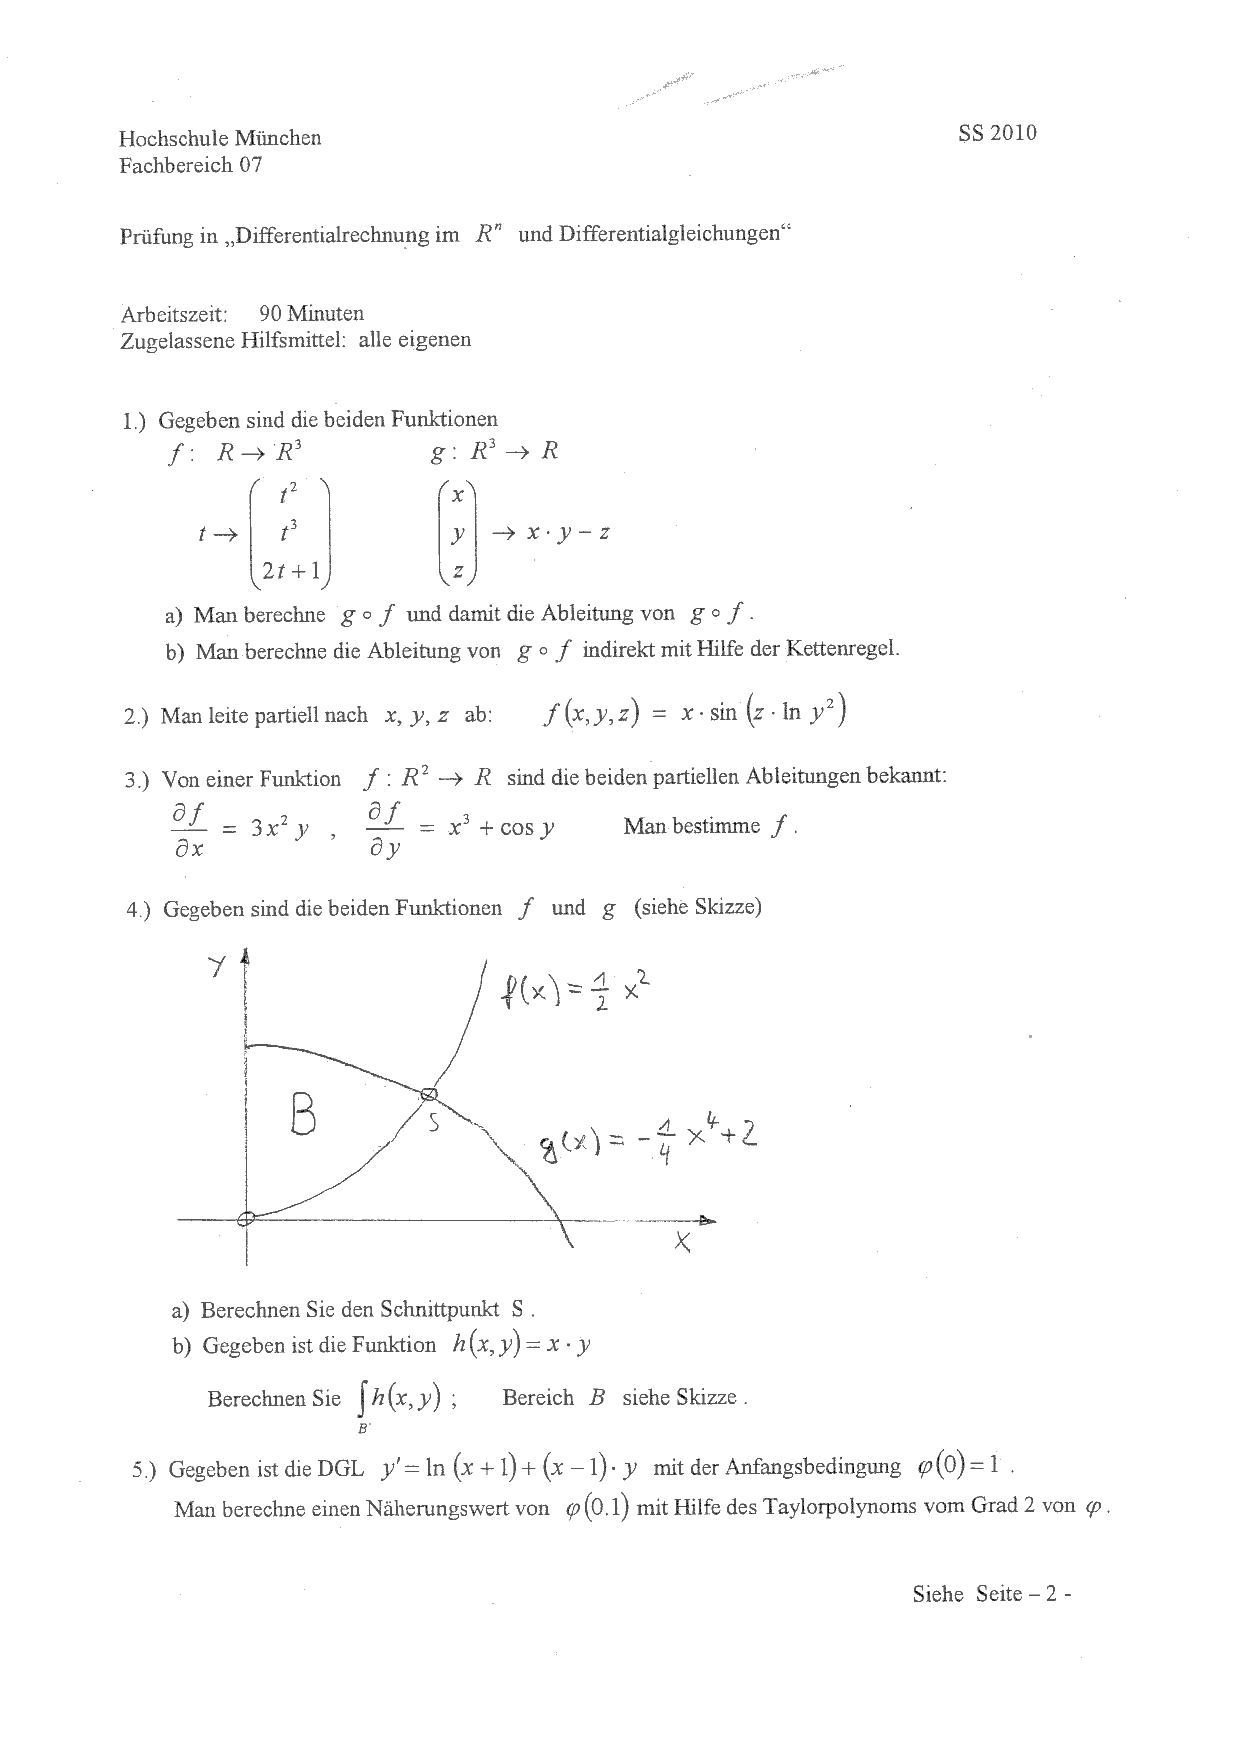
\includepdf[pages=-]{pruefungsangabe_diff_ss2010}

\section{Lösung für die Prüfung SS 2010}

\subsection{zu 1a)}
$ g\circ f) (t) = g\vektor{t^2\\t^2\\2t+1} = t^2 t^3 - (2t+1) = t^5 - 2t - 1$

$ (g\circ f)' (t) = 5 t^4 - 2$

\subsection{zu 1b)}
$ f'(t) = \vektor{2t\\3 t^2\\2}, g'\vektor{x\\y\\z} = \rbr{\frac{\delta g}{\dx},\frac{\delta g}{\dy},\frac{\delta g}{\dz}} = \rbr{y,x,-1} $

$g'(f(t)) \cdot f'(t) = g' \vektor{t^2\\t^3\\2t+1} \cdot \vektor{2t\\3t^2\\2} = \rbr{t^3, t^2, -1} \cdot \vektor{2t\\3t^2\\2} = 2t^4 \cdot 3t^4 - 2 = 5t^4 - 2 \checkmark$

\subsection{zu 2)}
$ f(x,y,z) = x\cdot \sin (z\cdot \ln y^2) = x \cdot \sin (2z \ln y)$

$ \frac{\df}{\dx} = \sin(z\cdot 2 \ln y)$

$\frac{\df}{\dy} = x\cdot \cos (z\cdot 2 \ln y) \cdot 2z \cdot \frac{1}{y} $

$\frac{\df}{\dz} = x\cdot \cos (z\cdot 2 \ln y) \cdot 2 \ln y$

\subsection{zu 3)}
Zum ersten Ausdruck: 
$ f(x,y) = 3y \cdot \frac{1}{3} x^3 + h(y) = yx^3 + h(y) $

Zum zweiten Ausdruck: 
$ f(x,y) = x^3 y + \sin y + g(x) $

$\Rightarrow h(y) = \sin y + g(x)$ In g(x) darf kein x vorkommen, also muss es eine Konstante sein: 
$ h(y) = \sin y + c$

$ f(x,y) = x^3y + \sin y + c $

\subsection{zu 4a)}
$ f(x) = g(x) $\\
$ \frac{1}{2} x^2 = -\frac{1}{4} x^4 + 2$ mit $x^2 = z$\\
$ \frac{1}{2} z = -\frac{1}{4} z^2 + 2 $\\
$ \Rightarrow z_1 = 2, z_2 = -4$\\
$z_2$ ist nicht möglich. $\Rightarrow z=2, x^2 = 2, x=\pm \sqrt{2} \Rightarrow x=\sqrt{2}$

\subsection{zu 4b)}
$ h(x,y) = x\cdot y$

$ \int_{B} h(x,y) 
= \int_{0}^{\sqrt{2}} \rbr{\int_{f(x)}^{g(x)} x \cdot y} dx 
= \int_{0}^{\sqrt{2}} \rbr{\sbr{\frac{1}{2} xy^2}_{y=f(x)}^{y=g(x)}} dx 
= \int_{0}^{\sqrt{2}} \frac{1}{2} x \sbr{\rbr{-\frac{1}{4} x^4 + 2}^2 - \rbr{\frac{1}{2} x^2}^2} dx 
= \int_{0}^{\sqrt{2}} \frac{1}{2} x \sbr{\frac{1}{16} x^8 + 4 - x^4 - \frac{1}{4} x^4} dx
= \frac{1}{2} \int_{0}^{\sqrt{2}} \rbr{\frac{1}{16} x^9 - \frac{5}{4} x^5 + 4x} dx
= \frac{1}{2} \sbr{\frac{1}{16} \cdot \frac{1}{10} x^{10} - \frac{5}{4} \cdot \frac{1}{6} x^6 + 4 \cdot \frac{1}{2} x^2}_0^{\sqrt{2}}
= 1.27
$

\subsection{zu 5)}
$ y' = \ln (x+1) + (x-1)\cdot y$ mit $ \varphi(0) = 1 $

Taylorpolynom: $\varphi(x) \approx \varphi(0) + \varphi'(0) \cdot x + \frac{\varphi''(0)}{2!} \cdot x^2$

$\varphi(0) = 1$

$\varphi'(0) = \ln(0+1) + (0-1) \cdot \varphi(0) = \ln 1 - 1 = -1$

$\varphi'(x) = \ln(x+1) + (x-1) \cdot \varphi(x)$

$\varphi''(x) = \frac{1}{x+1} + 1 \cdot \varphi(x) + (x-1)\cdot \varphi'(x)$

$ \varphi''(0) = 1 + 1 \cdot 1 - 1 \cdot - 1 = 3$

$\Rightarrow \varphi(x) \approx 1 - x + \frac{3}{2} x^2 $

$ \varphi(0.1) \approx 1 - 0.1 + \frac{3}{2} \cdot 0.01 = 0.915 $

\subsection{zu 6)}
P im u, v Koordinatensystem: 

u Wert: $\rbr{\cos \psi} + 2$ \profnote{Daheim nochmal anschauen}

v Wert: $ - \sin \psi$

$\psi$ ist die Bogenlänge (Der fette Bogen beim kleinen Kreis!).

$\psi = R \cdot \varphi = 3 \varphi$

$(u,v) = (2 + \cos \psi, -\sin \psi)$

Drehung um den Winkel $\varphi$: 

Drehmatrix: $\vektor{\cos \varphi & -\sin \varphi\\\sin \varphi & \cos \varphi}$

Koordinaten von P im xy-System:
 
$ \vektor{\cos \varphi & -\sin \varphi\\\sin \varphi & \cos \varphi} \vektor{2 + \cos 3 \varphi\\-\sin 3\varphi}
= \vektor{2\cos \varphi + \cos \varphi \cos 3 \varphi + \sin \varphi \sin 3 \varphi\\2\sin \varphi + \sin \varphi \cos 3 \varphi - \cos \varphi \sin 3 \varphi}
$

\subsection{zu 7)}
$y' = e^{\frac{y}{x}} + \frac{y}{x}$ mit $\varphi(1) = 2$. Wir substituieren $z = \frac{y}{x}$. 

$y = z \cdot x$

$y' = z' \cdot x + z $

Löse: $z' \cdot x + z = e^z + z$

$z'\cdot x = e^z$

$z' = \underbrace{\frac{1}{x}}_{f(x)} \cdot \underbrace{e^z}_{g(z)}$ (Typ getrennte Variable $\Rightarrow$ Gebrauchsanweisung)

$x_0 = 1$

$z(1)= \frac{y(1)}{1} = 2$

Rechne: 
$ \int_{1}^{x} f(t) dt = \int_{2}^{\psi(x)} \frac{1}{g(t)} dt $

$ \int_{1}^{x} \frac{1}{t} dt = \int_{2}^{\psi(x)} e^{-t} dt$

$ \sbr{\ln t}_1^t = \sbr{-e^{-t}}_2^{\psi(x)} $

$ \ln x = -e^{-\psi(x)} + e^{-2} $

$ e^{-\psi(x)} = e^{-2} - \ln x $

$ -\psi(x) = \ln(e^{-2} - \ln x) $

$ \psi(x) = -\ln(e^{-2} - \ln x) $ (Rücksubstitution!)

Lösung:
$ \varphi(x) = x \cdot \psi(x) = - x \ln(e^{-2} - \ln x)$

\renewcommand{\ldate}{2016-01-11}
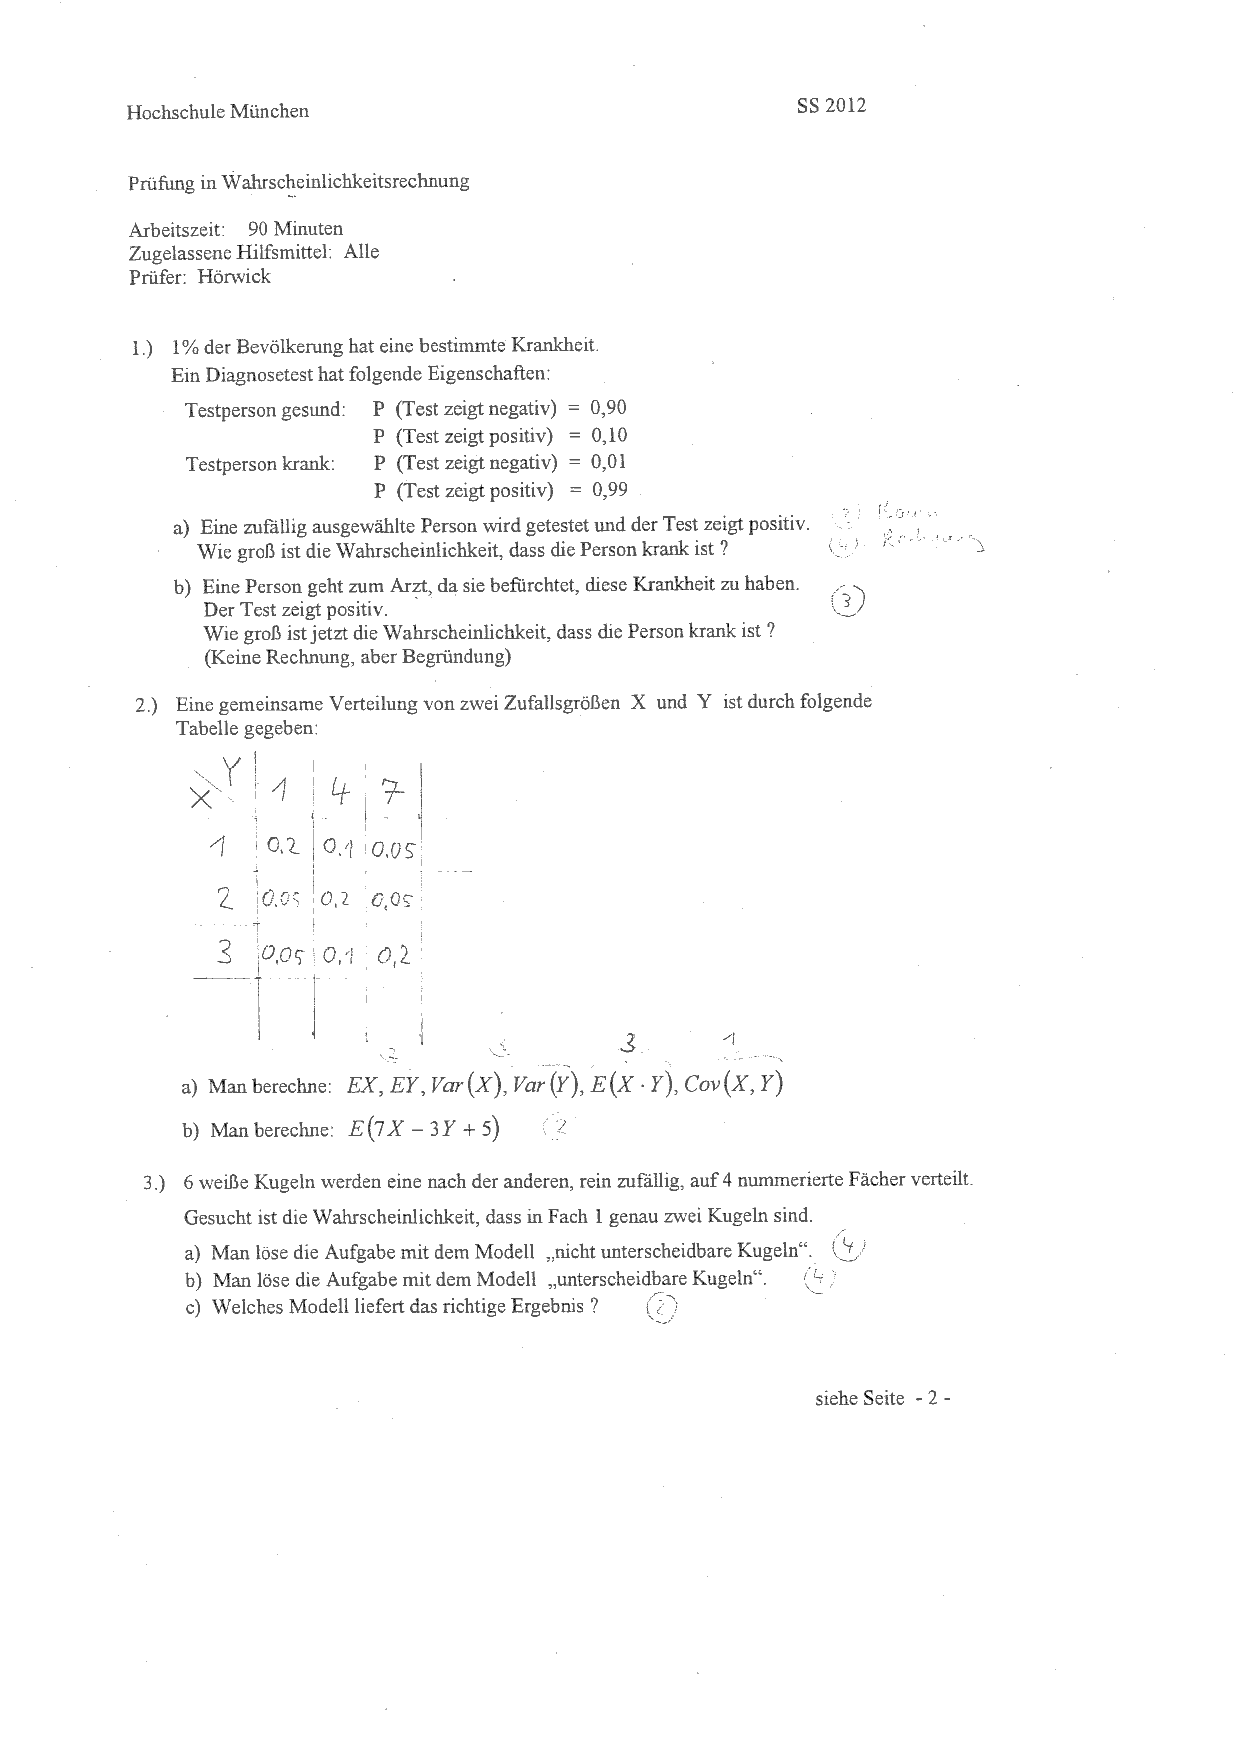
\includepdf[pages=-]{pruefungsangabe_wahrStat_ss2012}

\section{Lösung für die Prüfung SS 2012}

\subsection{zu 1)}
\includegraphicsdeluxe{baumZuSs20121.jpg}{Wahrscheinlichkeitsbaum}{Wahrscheinlichkeitsbaum}{fig:baumZuSs20121}

\subsubsection{zu 1a)}
A: Person krank\\
B: Test zeigt positiv
$P(A|B) = \frac{P\cap B}{P(B)} = \frac{0.01\cdot 0.99}{0.01\cdot 0.99 + 0.99\cdot 0.10} = 0.09$

\subsubsection{zu 1b)}
Jetzt ist die apriori Wahrscheinlichkeit, dass er krank ist, höher (vielleicht 0.1 statt 0.01). Damit ist die aposteriori Wahrscheinlichkeit, dass er krank ist, auch höher (vielleicht 0.5). 

\subsection{zu 2a)}

\begin{tabular}{|c|c|c|c|c|}
\hline X/Y & 1 & 4 & 7 &  \\ 
\hline 1 & 0.2 & 0.1 & 0.05 & 0.35 \\ 
\hline 2 & 0.05 & 0.2 & 0.05 & 0.3 \\ 
\hline 3 & 0.05 & 0.1 & 0.2 & 0.35 \\ 
\hline  & 0.3 & 0.4 & 0.3 &  \\ 
\hline 
\end{tabular} 

\begin{enumerate}
\item Immer multiplizieren Zeile mal Randwahrscheinlichkeit: $ EX = 1\cdot 0.35 + 2\cdot 0.3 + 3\cdot 0.35 = 2$
\item Wert mal Wahrscheinlichkeit: $ 1\cdot 0.3 + 4\cdot 0.4 + 7\cdot 0.3 = 4$
\item $EX^2 = 1^2 \cdot 0.35 + 2^2\cdot 0.3 + 3^2\cdot 0.35 = 1\cdot 0.35 + 4\cdot 0.3 + 9\cdot 0.35 = 4.7$\\
$EY^2 = 1\cdot 0.3 + 16\cdot 0.4 + 49\cdot 0.3 = 21.4 $\\
$Var(X) = E(X^2) - (EX)^2 = 4.7 - 4 = 0.7$\\
$Var(Y) = E(Y^2) - (EY)^2 = 21.4 - 16 = 5.4$\\
\item Nicht einfach multiplizieren. Ganze Tabelle durchmachen: $ E(X\cdot Y) = 
1\cdot 1\cdot 0.2 + 
1\cdot 4\cdot 0.1 + 
1\cdot 7\cdot 0.05 + 
2\cdot 1\cdot 0.05 + 
2\cdot 4\cdot 0.2 + 
2\cdot 7\cdot 0.05 + 
3\cdot 1\cdot 0.05 + 
3\cdot 4\cdot 0.1 + 
3\cdot 7\cdot 0.2 = 8.9
$
\item $ Cov(X,Y) = E(X\cdot Y) - EX\cdot EY = 8.9 - 2 \cdot 4 = 0.9$
\end{enumerate}

\subsection{zu 2b)}
$ E(7X - 3Y + 5) = 7 EX - 3 EY + 5 = 7\cdot 2 - 3\cdot 4 + 5 = 7$

\subsection{zu 3)}
\includegraphicsdeluxe{UrnenmodellSS20123.jpg}{Urnenmodell}{Urnenmodell}{fig:UrnenmodellSS20123}

\subsubsection{zu 3a)}
Anzahl der Möglichkeiten bei n Fächern und k Kugeln: 
$ \binom{n+k-1}{k}, n=4, k=6 $

alle Möglichkeiten: $ \binom{4+6-1}{6} = \binom 9 6 = \binom 9 3 = \frac{9\cdot 8\cdot 7}{1\cdot 2\cdot 3} = 84$

günstige Möglichkeiten, also 4 Kugeln auf 3 Fächer: $ \binom{3+4-1}{4} = \binom 6 4 = \binom 6 2 = \frac{6\cdot 5}{1\cdot 2} = 15$

$\Rightarrow P = \frac{15}{84} = 0.178 $

\subsubsection{zu 3b)}
Formel bei n Fächern und k Kugeln für die Anzahl der Möglichkeiten: $ n^k $

alle Fälle: $4^6 = 4096 $

günstige Fälle: $ \binom 6 2 \cdot 3^4 = \frac{6\cdot 5}{1\cdot 2} \cdot 3^4 = 1215 $   

$\Rightarrow P = \frac{1215}{4096} = 0.296$

\subsubsection{zu 3c)}
b ist richtig, weil a falsch ist. a ist falsch, weil nicht alle Möglichkeiten gleich wahrscheinlich sind. 
% \profnote{Student: Warum sind nicht alle Möglichkeiten gleich wahrscheinlich. Professor: Mei, das ist halt so.}

\subsection{zu 4)}
\profnote{Durchschnitt heißt immer Erwartungswert}
$ X_1 $ Anzahl der Nieten bis zum 1. Treffer. 

$ X_2 $ Anzahl der Nieten vom 1. bis zum 2. Treffer. 

$ \vdots $

$ X_{12} $ Anzahl der Nieten vom 11. bis zum 12. Treffer. 

$ Y = X_1 + X_2 + ... + X_{12}$

$EY = E \sum_{i=1}^{12} X_i = EX_1 + ... + EX_{12} = 12\cdot EX_1 = 12 \cdot \frac{1-P}{P} = 12\cdot \frac{1-0.2}{0.2} = 48$ 
Im Schnitt sind es also 48 Nieten bis zum 12. Treffer. Dadurch braucht man im Schnitt 60 Versuche bis zum 12. Treffer. 

\subsection{zu 5)}
X: Anzahl der Tests pro Gruppe (10).

$ P(X=1) = 0.95^{10} = 0.6 $

$ P(X=11) = 0.40 $

$ EX = 1\cdot 0.60 + 11\cdot 0.40 = 5.0$

Pro Gruppe im Schnitt 5.0 Tests. Pro Person werden also im Schnitt 0.5 Tests benötigt. \\

\subsection{zu 6)}
\includegraphicsdeluxe{UrneSS2012z6.jpg}{Urne}{Urne}{fig:UrneSS2012z6}

\subsubsection{zu 6a)}
Mit Rücklegen 5 mal ziehen: $ P(\textrm{5 mal weiß}) = \rbr{\frac{7}{8}}^5 = 0.513 $

$ P(\textrm{mindestens einmal schwarz}) = 1 - 0.513 = 0.487 $

\subsubsection{zu 6b)}
Ohne Rücklegen, mit der Abzählregel: 

alle Möglichkeiten: $ \binom 8 5 = \binom 8 3 = \frac{8\cdot 7\cdot 6}{1\cdot 2\cdot 3} = $

günstige Möglichkeiten: $ \binom 7 4 = \binom 7 3 = \frac{7\cdot 6\cdot 5}{1\cdot 2\cdot 3} = 35 $ 

$\Rightarrow P = \frac{35}{56} = 0.625 $

\profnote{Morgen nochmal eine Prüfung. Nächste Woche nichts mehr. Sprechstunde Dienstag 10-11 Uhr im R4.033.}
 % Vorlesung vom 18.06.2015
\renewcommand{\ldate}{2015-06-18}	% define lessiondate

% Angabe einbinden
% \includepdf[pages={1,3-5}]{Dateiname}

\section{Lösung zur Prüfung SS 2012}

\subsection{Aufgabe 1}

$ggT(91,55) \Rightarrow 91=1\cdot 55+36 \Rightarrow 55=1\cdot 36+19 \Rightarrow 36=1\cdot 19+17 \Rightarrow 19=1\cdot 17+2 \Rightarrow 17=8\cdot 2+1$\\
$1=17-8\cdot 2=17-8(19-17)=9\cdot 17-8\cdot 19=9(36-19)-8\cdot 19=9\cdot 36-17\cdot 19=9\cdot 36-17(55-36)=26\cdot 36-17\cdot 55=26(91-55)-17\cdot 55=26\cdot 91-43\cdot 55=1$

\subsection{Aufgabe 2}

\subsubsection{a}
$(\Z_{11},+,\cdot)$\\
I: $2x+y=0$ \\
II: $x-3y=10$\\
I-2 * II: $y+6y=-20 \Leftrightarrow 7y=2 (=13=24=35) \Rightarrow y=5$\\
in II: $x-3\cdot 5=10 \Rightarrow x=25=3$

\subsubsection{b}
$x=log(a) \Leftrightarrow 2^x=a$\\
$log(5) = ?$ (einfach ausprobieren)\\
$2, 2^2=4, 2^3=8, 2^4=16=5 \Leftrightarrow 2^4=5 \Rightarrow log(5)=4$\\
Kann man von jeder Zahl $\neq 0$ den Logarithmus bilden? Wir bilden dazu die Zweierpotenzen: $2, 2^2=4, 2^3=8, 2^4=16=5, 2^5=10, 2^6=9, 2^7=7, 2^8=3, 2^9=6, 2^{10}=1$. Das sind alle. Also kann man mit jeder Zahl den Logarithmus bilden.

\subsection{Aufgabe 3}

\subsubsection{a}
$\Z_{12}^* =\{1,5,7,11\}$\\ 
Wir bilden die Gruppentafel. In jeder Zeile bzw. Spalte darf und muss jede Zahl genau einmal vorkommen. 
\begin{tabular}{|c|c|c|c|c|}
\hline $\cdot$ & 1 & 5 & 7 & 11 \\ 
\hline 1 & 1 & 5 & 7 & 11 \\ 
\hline 5 & 5 & 1 & 11 & 7 \\ 
\hline 7 & 7 & 11 & 1 & 5 \\ 
\hline 11 & 11 & 7 & 5 & 1 \\ 
\hline 
\end{tabular} 

\subsubsection{b}
$\pi_1(5)\cdot \pi_2(7)\cdot \pi_3(x) = 1$\\
$7 \cdot  5 \cdot  \pi_3(x)=1$\\
$11 \cdot  \pi_3(x) = 1$\\
$\Rightarrow \pi_3(x)=11 \Rightarrow x=7$

\subsection{Aufgabe 4}
$\pi:
\begin{array}{cccccccc}
1 & 2 & 3 & 4 & 5 & 6 & 7 & 8 \\ 
\downarrow & \downarrow & \downarrow & \downarrow & \downarrow & \downarrow & \downarrow & \downarrow \\ 
3 & 7 & 1 & 5 & 2 & 8 & 4 & 6
\end{array} 
$\\
$c(i):=m(\pi(i)), m(i):=c(\pi^{-1}(i))$\\
$\pi^{-1}:
\begin{array}{cccccccc}
1 & 2 & 3 & 4 & 5 & 6 & 7 & 8 \\ 
\downarrow & \downarrow & \downarrow & \downarrow & \downarrow & \downarrow & \downarrow & \downarrow \\ 
3 & 5 & 1 & 7 & 4 & 8 & 2 & 6
\end{array} 
$\\
$m=(A,B,A,A,C,D,D,E)$\\
$c=(A,D,A,C,B,E,A,D)$\\
$\tilde{c}=(B,C,E,A,A,D,E,E)$\\
$\tilde{M}=(E,A,B,E,A,E,C,D)$\\

\subsection{Aufgabe 5}

\subsubsection{a}
Es gibt genau zwei Kanten mit ungeradem Grad. 

\subsubsection{b}
Lösung siehe Angabe. 

\subsection{Aufgabe 6}
Lassen wir weg, weil identisch mit anderem Jahrgang.

\subsection{Aufgabe 7}
Wir verteilen die $k=20$ Rosinen auf $n=10$ Fächer. Wir wählen Fach 1 aus: 
\includegraphicsdeluxe{rosinen_verteilung.jpg}{Die Rosinen werden verteilt}{fig:rosinen_verteilung} % Nr. 1
Alle Fälle: $10^{20}$\\
Günstige Fälle: $\binom{20}{2}\cdot 9^{18}$\\
$p=\frac{\textrm{günstige Fälle}}{\textrm{Nenner}}=\frac{\binom{20}{2}\cdot 9^{18}}{10^{20}}=...=0,285$

 % Vorlesung vom 22.06.2015
\renewcommand{\ldate}{2015-06-22}	% define lessiondate

\section{Einzelne Aufgaben}

\subsection{Dominosteine in 3xn-Feld unterbringen}
Wie viele Möglichkeiten a(n) gibt es 1x2-Steine anzuordnen? Wenn n ungerade ist, geht es nicht. 
\includegraphicsdeluxe{dominofelddarstellung.jpg}{Wie kann man die 1x2 Steine im Feld unterbringen?}{fig:dominofelddarstellung} % Nr. 1
Wenn man die Anfänge in Abb. \ref{fig:dominofelddarstellung} betrachtet kommt man auf folgende Formeln für die Möglichkeiten: 

\begin{itemize}
\item $a(n)=a(n-2)+2 b(n)$
\item $b(n)=a(n-2)+b (n-2)$
\end{itemize}

\begin{tabular}{|c|c|c|c|c|}
\hline n & 2 & 4 & 6 & 8 \\ 
\hline a(n) & 3 & $3+2\cdot 4=11$ & $11+2\cdot 15=41$ & $41+2\cdot 56=153$ \\ 
\hline b(n) & 1 & $3+1=4$ & $11+4=15$ & $41+15=56$ \\ 
\hline 
\end{tabular} 

\subsection{Rechnen im $\Z_{11}$}
Wir rechnen in $(\Z_{11},+,\cdot)$. 11 ist eine Primzahl also ist das ein Körper. 

\subsubsection{Lineares Gleichungssystem}
I: $x+3y=8$\\
II: $2x+y=4$\\

II-2I: $y-6y=4-16$\\
$-5y=-12$\\
$5y=12=23=34=45$\\
$\Rightarrow y=9$\\

in I: $x+3\cdot 9=8$\\
$x=8-27=-19$\\
$x=3$

\subsubsection{Quadratische Gleichung}
$x^2+4x=10$ mit $(a+b)^2 = a^2+2ab+b^2 \Rightarrow b=2$\\
$x^2+4x+w^2=10+2^2$\\
$(x+2)^2=14=3$\\
Die Lösungen finden wir mittels Ausprobieren: 
$2^2=4, 3^2=9, 4^2=16=5,$ \textbf{$5^2=25=3$}\\
$x+2=\pm 5$\\
$x_1 + 2 = 5 \Rightarrow x_1=3$\\
$x_2+2=-5 \Rightarrow x_2=-7=4$\\

\subsection{Kombinatorikaufgabe}
10 Ehepaare sitzen an einem langen Tisch. Auf einer Seite die Männer, auf der anderen die Frauen. Wie groß ist die Wahrscheinlichkeit, dass sich kein Ehepaar gegenüber sitzt? \\
Das klingt nach Permutationen: \\
$
\begin{array}{ccccccc}
\textrm{Männer} & 1 & 2 & 3 & 4 & ... & 10 \\ 
 & \downarrow & \downarrow & \downarrow & \downarrow & \downarrow & \downarrow \\ 
\textrm{Frauen} & 3 & 4 & 7 & 10 & ... & 5
\end{array} 
$\\
Damit kann man die Aufgabe neu formulieren: Wie groß ist die Wahrscheinlichkeit, dass die Permutationen keinen Fixpunkt hat?\\
alle Permutationen: n!\\
Permutationen ohne Fixpunkt: $a(n)=n!\underbrace{(1-\frac{1}{1!}+\frac{1}{2!}-\frac{1}{3!}+...+(-1)^n \frac{1}{n!})}_{\approx e^{-1}} \approx n! e^{-1}= \frac{10!}{e}$\\
P(kein Fixpunkt)$=\frac{\textrm{günstige Fälle}}{\textrm{alle Fälle}}=\frac{\frac{n!}{e}}{n!}=\frac{1}{e}=0,367$

\subsection{Einheitengruppe}
$(\Z_{16}^* ,\cdot)$ Einheitengruppe (teilerfremd zu 16): $\Z_{16}^*  = \{1,3,5,7,9,11,13,15\}$\\
Jetzt machen wir einen Code c über $\Z_{16}^* $.\\
$c=\{(a,b,c) : a b c = 1, a,b,c \in \Z_{16}^* \}$\\
\paragraph{Ergänze $(5,11,\cdot)$} zu einem Codewort.\\
$5\cdot 11\cdot x=1$\\
$55 x = 1$\\
$7 x = 1$ \\
Jetzt probieren wir die Werte aus der o.g. Einheitengruppe aus:\\
$7\cdot 3=21=5$\\
$7\cdot 3=35=3$\\
$7\cdot 7=49=1$\\
$\Rightarrow x=7$

\paragraph{Aus wie vielen Elementen besteht der Code?}
$(a,b,\cdot)$ mit a,b beliebig wählen und $\cdot$ rechnen wir aus.
Für a und b gibt es jeweils 8 Möglichkeiten (Anzahl der Elemente der Einheitengruppe), also 64 Elemente. Der Code hat also 64 Codewörter. 

\subsection{Verschlüsseln und Entschlüsseln mit Permutationen}
\paragraph{Wir haben eine gegebene Permutation}
$\pi: 
\begin{array}{ccccccc}
1 & 2 & 3 & 4 & 5 & 6 & 7 \\ 
\downarrow & \downarrow & \downarrow & \downarrow & \downarrow & \downarrow & \downarrow \\ 
3 & 7 & 1 & 5 & 4 & 2 & 6
\end{array} 
$
\paragraph{Suche die inverse Permutation}
$\pi^{-1}: 
\begin{array}{ccccccc}
1 & 2 & 3 & 4 & 5 & 6 & 7 \\ 
\downarrow & \downarrow & \downarrow & \downarrow & \downarrow & \downarrow & \downarrow \\ 
3 & 6 & 1 & 5 & 4 & 7 & 2
\end{array} 
$

\paragraph{Damit kann man Wörter der Länge 7 verschlüsseln.}
$c(i):=m(\pi(i))$\\

\paragraph{Verschlüssle $m=(C,A,B,C,D,E,A)$}
$\Rightarrow c=(B,A,C,D,C,A,E)$

\paragraph{Entschlüssle c (mit $\pi^{-1}$)}
$m(i) := c(\pi^{-1}(i))$\\
$m=(C,A,B,C,D,E,A) \checkmark$

\subsection{Graphentheorie}
Hat der gegebene Graph (Abb. \ref{fig:aufgaben_graphen6}) einen eulerschen Kreis oder eine eulersche Linie? 
\includegraphicsdeluxe{aufgaben_graphen6.jpg}{Eulersche Linie und eulerscher Kreis}{fig:aufgaben_graphen6} % Nr. 2

\subsubsection{eulersche Linie}
Es gibt genau zwei Knoten (A, E) mit ungeradem Grad $\Rightarrow$ eulersche Linie (rot). Beim Einzeichnen muss man bei einem Knoten mit ungeradem Grad (z.B. A oder E) starten! 

\subsubsection{eulerscher Kreis}
Füge eine zusätzliche Kante ein, damit ein eulerscher Kreis (nur gerade Grade) entsteht (blau). 

 % Vorlesung vom 25.06.2015
\renewcommand{\ldate}{2015-06-25}	% define lessiondate

% Angabe einbinden
% \includepdf[pages={1,3-5}]{Dateiname}

\section{Lösung zur Prüfung SS 2008}

\subsection{Aufgabe 1}
$n=1: $ linke Seite: 1, rechte Seite 1 $\checkmark$\\
Zeige: $\sum_{k=1}^{n+1}=\frac{(n+1)^2 (n+2)^2}{4} \Leftrightarrow \frac{n^2 (n+1)^2}{4}+(n+1)=\frac{(n+1)^2 (n+2)^2}{4}$
$\Leftrightarrow (n+1)^3=\frac{(n+1)^2 (n+2)^2 - n^2 (n+1)^2}{4} \Leftrightarrow (n+1) = \frac{(n+2)^2 - n^2}{4} = \frac{n^2+4n+4-n^2}{4} \Rightarrow n+1=n+1$

\subsection{Aufgabe 2}\index{Euklidischer Algorithmus}
ggT(385,595)\\

\begin{tabular}{|c|c|c|c|c|c|}
\hline a & b & q & r & x & y \\ 
\hline 595 & 385 & 1 & 210 &  &  \\ 
\hline 385 & 210 & 1 & 175 &  &  \\ 
\hline 210 & 175 & 1 & 35 & 1 &  \\ 
\hline 175 & 35 & 5 & 0 & 0 & 1 \\ 
\hline  &  &  &  &  &  \\ 
\hline 
\end{tabular}\\
 
\marginpar{$y=x_{i+1} - q_i \cdot  y_{i+1}$}
$\Rightarrow ggT = 35 ... = 2 \cdot  595 - 3 \cdot  385 \Rightarrow 350 = 10 \cdot  35 = 20 \cdot  595 - 30 \cdot  385$ 

\subsection{Aufgabe 3}

\subsubsection{a}
$(\Z_{15}^* ,\cdot) \Rightarrow \{1,2,4,7,8,11,13,14\}$\\

\begin{tabular}{|c|c|c|c|c|c|c|c|c|}
\hline $\cdot$ & 1 & 2 & 4 & 7 & 8 & 11 & 13 & 14 \\ 
\hline 1 & 1 & 2 & 4 & 7 & 8 & 11 & 13 & 14 \\ 
\hline 2 & 2 & 4 & 8 & 14 & 1 & 7 & 11 & 13 \\ 
\hline 4 & 4 & 8 & 1 & 13 & 2 & 14 & 7 & 11 \\ 
\hline 7 & 7 & 14 & 13 & 4 & 11 & 2 & 1 & 8 \\ 
\hline 8 & 8 & 1 & 2 & 11 & 4 & 13 & 14 & 7 \\ 
\hline 11 & 11 & 7 & 14 & 2 & 13 & 1 & 8 & 4 \\ 
\hline 13 & 13 & 11 & 7 & 1 & 14 & 8 & 4 & 2 \\ 
\hline 14 & 14 & 13 & 11 & 8 & 7 & 4 & 2 & 1 \\ 
\hline 
\end{tabular} \\
Weil es sich hierbei um eine Gruppe handelt, ist die Tafel symmetrisch zur Diagonalen. Außerdem kommt in jeder Spalte und Zeile jede Zahl nur einmal vor. 

\subsubsection{b}
$11 x^2=14 \Leftrightarrow x^2=11\cdot 14=4 \Rightarrow x=2,7,8,13$
Gleichung lösen und dann zu x passende Werte aus der Tafel finden. 

\subsubsection{c}
$
\begin{array}{ccccccccc}
\pi & 1 & 2 & 4 & 7 & 8 & 11 & 13 & 14 \\ 
\downarrow & \downarrow & \downarrow & \downarrow & \downarrow & \downarrow & \downarrow & \downarrow & \downarrow \\ 
\pi_{1} & 4 & 7 & 11 & 14 & 13 & 8 & 1 & 2 \\
\pi_{2} & 11 & 14 & 8 & 2 & 1 & 13 & 4 & 7 \\
\pi_{3} & 8 & 2 & 13 & 7 & 4 & 1 & 11 & 14 \\
\pi_{4} & 13 & 7 & 1 & 14 & 11 & 4 & 8 & 2 \\
\end{array}
$\\
$c = \{(a,b,c,d) : \pi_{1}(a) \cdot  \pi_{2}(b) \cdot  \pi_{3}(c) \cdot  \pi_{4}(d) = 1 \}$
d ist frei wählbar. Für a, b, c gibt es jeweils 8 Möglichkeiten $\Rightarrow$ Anzahl der Wörter: $8^3=512$

\paragraph{Ergänze $(7,13,11,\cdot)$:}
$\pi_{1}(7) \cdot  \pi_{2}(13) \cdot  \pi_{3}(11) \cdot  \pi_{4}(x)=1$\\
$14 \cdot  4 \cdot  1 \cdot  \pi_{4}(x)=1$\\
$11 \cdot  \pi_{4}(x)=1$\\
$\Rightarrow \pi_{4}(x)=11 \Rightarrow x=8$

\subsection{Aufgabe 4}

\subsubsection{a}
$28^{52} = 1$ 

\subsubsection{b}\index{schnelle Exponentation}
$28^{34}=?$\\
$34=2^5 + 2^1$ mod 53\\
$28^{(2^0)} = 28$\\
$28^{(2^1)} = 784 = 42$\\
$28^{(2^2)} = 42^2 = 1764 = 15$\\
$28^{(2^3)} = 15^2 = 225 = 13$\\
$28^{(2^4)} = 13^2 = 169 = 10$\\
$28^{(2^5)} = 10^2 = 100 = 47$\\
$28^{34} = 28^{2^5+2^1}= 28^{(2^5)} \cdot  28^{(2^1)} = 47 \cdot  42 = 1974 = 13$

\subsection{Aufgabe 5}

\subsubsection{a} 
7 Personen (Schubfachprinzip)\index{Schubfachprinzip}

\subsubsection{b} 
Es gibt 3n gerade, 3n ungerade Elemente. Die ungeraden sollen nun an einer geraden Stelle stehen. Daher gibt es $(3n)!$ Möglichkeiten ungerade Elemente auf geraden Stellen platzieren. Bei den geraden ist es genauso: $(3n)!$. Insgesamt also: $(3n)! \cdot  (3n)!$

\subsubsection{c} 
Es gibt 5 unterschiedliche Buchstaben (5 x A , 2 x B, 1 x C, 1 x D, 2 x R) und 11 Stellen. Man kann das mit dem Multinomialkoeffizienten berechnen (allgemein): $\binom{n}{a,b,c} = \frac{n!}{a! b! c!} \Rightarrow \binom{11!}{5,2,1,1,2} = \frac{11!}{5! 2! 1! 1! 2!} = \binom{11!}{5! 4} = \binom{11 \cdot  10 \cdot  9 \cdot  8 \cdot  7 \cdot  6}{4} = 11 \cdot  10 \cdot  9 \cdot  2 \cdot  7 \cdot  6 = 83160$

 % Vorlesung vom 29.06.2015
\renewcommand{\ldate}{2015-06-29}	% define lessiondate

\section{Einzelne Aufgaben}

\subsection{Siebformel}\index{Siebformel}

$|A_1 \cup A_2 \cup A_3 \cup A_4| = |A_1| + |A_2| + |A_3| + |A_4| - [|A_1 \cap A_2| + |A_1 \cap A_3| + |A_1 \cap A_4| + |A_2 \cap A_3| + |A_2 \cap A_4| + |A_3 \cap A_4|] + [|A_2 \cap A_3 \cap A_4| + |A_1 \cap A_3 \cap A_4| + |A_1 \cap A_2 \cap A_4| + |A_1 \cap A_2 \cap A_3|] - [|A_1 \cap A_2 \cap A_3 \cap A_4|]$

\subsubsection{Beispiel}
\includegraphicsdeluxe{siebformel_mengen.jpg}{Auf diese Menge wenden wir die Siebformel an}{fig:siebformel_mengen} % Nr. 1

\subsubsection{Berechnung}
$[8+8+8+8]-[5+3+2+4+4+4]+[2+1+2+2]-[1]=32-22+7-1=16$

\subsection{Symmetriegruppe eines Rechtecks}
Eine Kongruenzabbildung (Drehung, Spiegelung), die das Rechteck auf sich selbst abbildet. Wir bilden die dazugehörige Gruppentafel:

\begin{tabular}{|c|c|c|c|c|}
\hline $\circ$ & id & d & s & t \\ 
\hline id & id & d & s & t \\ 
\hline d & d & id & $d \circ s = t$ & s \\ 
\hline s & s & t & id & d \\ 
\hline t & t & s & d & id \\ 
\hline 
\end{tabular} 
\\
Eine Zelle machen wir ausführlich: $d \circ s: A \rightarrow D, B \rightarrow C, C \rightarrow B, D \rightarrow A$ Was ist jetzt $d \circ s$? Die Spiegelung an t. 

\includegraphicsdeluxe{symmgruppe_rechteck.jpg}{Spiegelungen an s und t, Drehung d um 180, Drehung id um 360}{fig:symmgruppe_rechteck} % Nr. 2

\subsection{RSA-Algorithmus}\index{RSA}
Wir brauchen zwei Primzahlen: $p=5, q=7$\\
Dann müssen wir das n ausrechnen: $n=p \cdot  q=35$\\
Wir brauchen die eulersche Phi-Funktion: $\varphi(n)=\varphi(35)=4\cdot 6=24$\\
Jetzt wählen wir ein e: $1 < e < 24$ mit $ggT(e,24)=1$. Wir wählen $e=11$\\
Berechne d mit $e \cdot  d \equiv 1$ mod $\varpi(n)$\\
$11 \cdot  d \equiv 1$ mod $24$\\
Mit euklidischem Algorithmus: ggT(11,24)\\
$24=2\cdot 11+2$\\
$11=5\cdot 2+1$\\
Jetzt Kombination bilden: $1=11-5\cdot 2=11-5(24-2\cdot 11)=11\cdot 11-5\cdot 24=1$\\
$\Rightarrow 11\cdot 11\equiv 1$ mod $24$\\
$11\cdot d\equiv1$ mod $24$\\
Das Inverse von d ist zufällig auch 11. 

\paragraph{Schlüssel}
öffentlich: n,e\\
geheim: d\\
Klartext: $m=4$\\
$c=m^e$ mod n\\
$c=4^{11}$ mod 35\\
$4194304=9$

\paragraph{entschlüsseln:}
$m=c^d$ mod n\\
$m=9^{11}$ mod 35\\
$m=9^{11}=9^5\cdot 9^6=59049 \cdot  531441 = 4 \cdot  1 = 4$

\section{Prüfungsstoff}
Prüfungen SS2008, SS2010, SS2011, SS2012, WS1415\\
Außerdem: Aufgaben von heute, Induktionsbeweis Dominosteine, Lineares Gleichungssystem mod x, Quadratische Gleichung mod x, Permutationen (mit und ohne Fixpunkt), Codes (Gruppen mit und ohne  Permutationen), Graphen (eulersche Linie, eulerscher Kreis)

 % Vorlesung vom 29.06.2015
\renewcommand{\ldate}{Anhang}	% define lessiondate

\section{Hilfsmittel für die Prüfung}
\subsection{Eulerkreis und Eulertour}
\paragraph{Der Eulerkreis} enthält alle Kanten des Graphen G \textbf{genau einmal}. Der Eulerkreis kann gezeichnet werden ohne abzusetzen. Es gilt: 
\begin{itemize}
\item G ist eulersch,
\item G ist zusammenhängend und jeder Knoten hat geraden Grad.
\end{itemize}
\paragraph{Eine Eulertour} bzw. offene eulersche Linie nennt man einen Weg, der \textbf{kein Kreis} ist, wenn jede Kante darin \textbf{genau einmal} vorkommt. 

G ist \textbf{offene eulersche Linie} $\Leftrightarrow$ G hat \textbf{genau zwei Knoten} mit \textbf{ungeradem Grad}

\subsection{Chinesischer Restsatz} 
Seien $m_1, m_2, ..., m_n$  \textbf{teilerfremde} natürliche Zahlen und $a_1, a_2, ..., a_n \in \Z$ beliebig $\exists x\in \Z$ mit: \\

$
\left.
\begin{matrix}
x\equiv a_1 \textrm{ mod } m_1\\
x\equiv a_2 \textrm{ mod } m_2\\
\vdots\\
x\equiv a_n \textrm{ mod } m_n\\
\end{matrix}
\right\rbrace
$ simultane Kongruenz\\

$m=m_1\cdot m_2\cdot ...\cdot m_n$\\
$M_i=\frac{m_1\cdot m_2\cdot ...\cdot m_n}{m_i}=\frac{m}{m_i}$\\

\subsection{Permutationen}
\subsubsection{Anzahl Permutationen ohne Fixpunkte}
\paragraph{genaue Berechnung}
$a(n)=n!\underbrace{(1-\frac{1}{1!}+\frac{1}{2!}-\frac{1}{3!}+...+(-1)^n \frac{1}{n!})}_{\approx e^{-1}}$
\paragraph{Nährungslösung}
$a(n) \approx n! e^{-1}= \frac{n!}{e}$
\paragraph{Wahrscheinlichkeit kein Fixpunkt}
$P=\frac{\textrm{günstige Fälle}}{\textrm{alle Fälle}} = \frac{a(n)}{n!}$

\subsection{ggT} Seien $a,b \in \Z$ mit $a \neq 0$. Seien q und r Zahlen mit $b=qa+r \Rightarrow ggT(b,a)=ggT(a,r)$.

\subsubsection{euklidischer Algorithmus} Der euklidische Algorithmus ist ein Algorithmus aus dem mathematischen Teilgebiet der Zahlentheorie. Mit ihm lässt sich der größte gemeinsame Teiler zweier natürlicher Zahlen a und b berechnen. Als erstes berechnet man a mod b. Dabei erhält man das ganzzahlige Ergebnis der Division und den Rest r. Das macht man so lange, bis man für den Rest 0 erhält. Das aktuelle b ist dann der ggT(a,b). Tabellarisch kann man den Algorithmus wie im folgenden Beispiel durchführen ggT(128,34):

\begin{tabular}{|c|c|c|c|}
\hline a & b & q & r \\ 
\hline 128 & 34 & 3 & 26 \\ 
\hline 34 & 26 & 1 & 8 \\ 
\hline 26 & 8 & 3 & 2 \\ 
\hline 8 & 2 & 4 & 0 \\ 
\hline 
\end{tabular} 

\subsubsection{Erweiterter euklidischer Algorithmus}
Der erweiterte euklidische Algorithmus ist ein Algorithmus aus dem mathematischen Teilgebiet der Zahlentheorie. Er berechnet neben dem größten gemeinsamen Teiler ggT(a,b) zweier natürlicher Zahlen a und b noch zwei ganze Zahlen x und y, die die folgende Gleichung erfüllen: $ggT(a,b) = x \cdot a + y \cdot b$. 

Den erweiterten euklidischen Algorithmus startet man unten auf der rechten Seite der Tabelle. Das Ergebnis steht dann rechts in der obersten Zeile. Dabei ist $x_i=y_{i+1}$ und $y_i = x_{i+1} - q_i * y_{i+1}$:

\begin{tabular}{|c|c|c|c||c|c|}
\hline a & b & q & r & x & y \\ 
\hline 128 & 34 & 3 & 26 & 4 & -15 \\ 
\hline 34 & 26 & 1 & 8 & -3 & 4 \\ 
\hline 26 & 8 & 3 & 2 & 1 & -3 \\ 
\hline 8 & 2 & 4 & 0 & 0 & 1 \\ 
\hline 
\end{tabular} 

\subsection{schnelle Exponentation}\index{schnelle Exponentation}
Im Zahlenkörper ($\Z_{\textbf{53}},+,\cdot$) berechne man:
$28^{34}=?$\\
$34=2^5 + 2^1$ mod \textbf{53}\\
$28^{(2^0)} = 28$\\
$28^{(2^1)} = 784 = \textbf{\underline{42}}$\\
$28^{(2^2)} = \textbf{42}^2 = 1764 = \textbf{15}$\\
$28^{(2^3)} = \textbf{15}^2 = 225 = \textbf{13}$\\
$28^{(2^4)} = \textbf{13}^2 = 169 = \textbf{10}$\\
$28^{(2^5)} = \textbf{10}^2 = 100 = \textbf{\underline{47}}$\\
$28^{34} = 28^{2^5+2^1}= 28^{(2^5)} \cdot  28^{(2^1)} = \textbf{\underline{47}} \cdot  \textbf{\underline{42}} = 1974 = 13$

\subsection{$\Z_n^*$}
Wir bezeichnen die Menge derjenigen Restklassen von $\Z_n$, die ein multiplikatives Inverses haben, mit $\Z_n^*$. In $\Z_n^*$ liegen also genau diejenigen Restklassen [a] von $\Z_n$ mit $ggT(a,n)=1$.
Die Restklassen [1] und [n-1] sind stets in $\Z_n^*$ enthalten, denn beide sind teilerfremd zu n. 

$\Z_n^*$ ist abgeschlossen bezüglich Multiplikation $\Rightarrow$ $[a]\cdot [b]$ liegt wieder in $\Z_n^*$. $\Z_n^*$ ist eine \textbf{Gruppe} $\Rightarrow$ Es gilt das Assoziativgesetz, es gibt ein neutrales Element und jedes Element hat ein Inverses. 

\subsubsection{$\Z_{4}^*$}
\begin{tabular}{|c|c|c|}
\hline $\cdot$  & 1 & 3\\
\hline 1 & 1 & 3\\
\hline 3 & 3 & 1\\
\hline
\end{tabular}


\subsubsection{$\Z_{5}^*$}
\begin{tabular}{|c|c|c|c|c|}
\hline $\cdot$  & 1 & 2 & 3 & 4\\
\hline 1 & 1 & 2 & 3 & 4\\
\hline 2 & 2 & 4 & 1 & 3\\
\hline 3 & 3 & 1 & 4 & 2\\
\hline 4 & 4 & 3 & 2 & 1\\
\hline
\end{tabular}


\subsubsection{$\Z_{6}^*$}
\begin{tabular}{|c|c|c|}
\hline $\cdot$  & 1 & 5\\
\hline 1 & 1 & 5\\
\hline 5 & 5 & 1\\
\hline
\end{tabular}


\subsubsection{$\Z_{7}^*$}
\begin{tabular}{|c|c|c|c|c|c|c|}
\hline $\cdot$  & 1 & 2 & 3 & 4 & 5 & 6\\
\hline 1 & 1 & 2 & 3 & 4 & 5 & 6\\
\hline 2 & 2 & 4 & 6 & 1 & 3 & 5\\
\hline 3 & 3 & 6 & 2 & 5 & 1 & 4\\
\hline 4 & 4 & 1 & 5 & 2 & 6 & 3\\
\hline 5 & 5 & 3 & 1 & 6 & 4 & 2\\
\hline 6 & 6 & 5 & 4 & 3 & 2 & 1\\
\hline
\end{tabular}


\subsubsection{$\Z_{8}^*$}
\begin{tabular}{|c|c|c|c|c|}
\hline $\cdot$  & 1 & 3 & 5 & 7\\
\hline 1 & 1 & 3 & 5 & 7\\
\hline 3 & 3 & 1 & 7 & 5\\
\hline 5 & 5 & 7 & 1 & 3\\
\hline 7 & 7 & 5 & 3 & 1\\
\hline
\end{tabular}


\subsubsection{$\Z_{9}^*$}
\begin{tabular}{|c|c|c|c|c|c|c|}
\hline $\cdot$  & 1 & 2 & 4 & 5 & 7 & 8\\
\hline 1 & 1 & 2 & 4 & 5 & 7 & 8\\
\hline 2 & 2 & 4 & 8 & 1 & 5 & 7\\
\hline 4 & 4 & 8 & 7 & 2 & 1 & 5\\
\hline 5 & 5 & 1 & 2 & 7 & 8 & 4\\
\hline 7 & 7 & 5 & 1 & 8 & 4 & 2\\
\hline 8 & 8 & 7 & 5 & 4 & 2 & 1\\
\hline
\end{tabular}


\subsubsection{$\Z_{10}^*$}
\begin{tabular}{|c|c|c|c|c|}
\hline $\cdot$  & 1 & 3 & 7 & 9\\
\hline 1 & 1 & 3 & 7 & 9\\
\hline 3 & 3 & 9 & 1 & 7\\
\hline 7 & 7 & 1 & 9 & 3\\
\hline 9 & 9 & 7 & 3 & 1\\
\hline
\end{tabular}


\subsubsection{$\Z_{11}^*$}
\begin{tabular}{|c|c|c|c|c|c|c|c|c|c|c|}
\hline $\cdot$  & 1 & 2 & 3 & 4 & 5 & 6 & 7 & 8 & 9 & 10\\
\hline 1 & 1 & 2 & 3 & 4 & 5 & 6 & 7 & 8 & 9 & 10\\
\hline 2 & 2 & 4 & 6 & 8 & 10 & 1 & 3 & 5 & 7 & 9\\
\hline 3 & 3 & 6 & 9 & 1 & 4 & 7 & 10 & 2 & 5 & 8\\
\hline 4 & 4 & 8 & 1 & 5 & 9 & 2 & 6 & 10 & 3 & 7\\
\hline 5 & 5 & 10 & 4 & 9 & 3 & 8 & 2 & 7 & 1 & 6\\
\hline 6 & 6 & 1 & 7 & 2 & 8 & 3 & 9 & 4 & 10 & 5\\
\hline 7 & 7 & 3 & 10 & 6 & 2 & 9 & 5 & 1 & 8 & 4\\
\hline 8 & 8 & 5 & 2 & 10 & 7 & 4 & 1 & 9 & 6 & 3\\
\hline 9 & 9 & 7 & 5 & 3 & 1 & 10 & 8 & 6 & 4 & 2\\
\hline 10 & 10 & 9 & 8 & 7 & 6 & 5 & 4 & 3 & 2 & 1\\
\hline
\end{tabular}


\subsubsection{$\Z_{12}^*$}
\begin{tabular}{|c|c|c|c|c|}
\hline $\cdot$  & 1 & 5 & 7 & 11\\
\hline 1 & 1 & 5 & 7 & 11\\
\hline 5 & 5 & 1 & 11 & 7\\
\hline 7 & 7 & 11 & 1 & 5\\
\hline 11 & 11 & 7 & 5 & 1\\
\hline
\end{tabular}


\subsubsection{$\Z_{13}^*$}
\begin{tabular}{|c|c|c|c|c|c|c|c|c|c|c|c|c|}
\hline $\cdot$  & 1 & 2 & 3 & 4 & 5 & 6 & 7 & 8 & 9 & 10 & 11 & 12\\
\hline 1 & 1 & 2 & 3 & 4 & 5 & 6 & 7 & 8 & 9 & 10 & 11 & 12\\
\hline 2 & 2 & 4 & 6 & 8 & 10 & 12 & 1 & 3 & 5 & 7 & 9 & 11\\
\hline 3 & 3 & 6 & 9 & 12 & 2 & 5 & 8 & 11 & 1 & 4 & 7 & 10\\
\hline 4 & 4 & 8 & 12 & 3 & 7 & 11 & 2 & 6 & 10 & 1 & 5 & 9\\
\hline 5 & 5 & 10 & 2 & 7 & 12 & 4 & 9 & 1 & 6 & 11 & 3 & 8\\
\hline 6 & 6 & 12 & 5 & 11 & 4 & 10 & 3 & 9 & 2 & 8 & 1 & 7\\
\hline 7 & 7 & 1 & 8 & 2 & 9 & 3 & 10 & 4 & 11 & 5 & 12 & 6\\
\hline 8 & 8 & 3 & 11 & 6 & 1 & 9 & 4 & 12 & 7 & 2 & 10 & 5\\
\hline 9 & 9 & 5 & 1 & 10 & 6 & 2 & 11 & 7 & 3 & 12 & 8 & 4\\
\hline 10 & 10 & 7 & 4 & 1 & 11 & 8 & 5 & 2 & 12 & 9 & 6 & 3\\
\hline 11 & 11 & 9 & 7 & 5 & 3 & 1 & 12 & 10 & 8 & 6 & 4 & 2\\
\hline 12 & 12 & 11 & 10 & 9 & 8 & 7 & 6 & 5 & 4 & 3 & 2 & 1\\
\hline
\end{tabular}


\subsubsection{$\Z_{14}^*$}
\begin{tabular}{|c|c|c|c|c|c|c|}
\hline $\cdot$  & 1 & 3 & 5 & 9 & 11 & 13\\
\hline 1 & 1 & 3 & 5 & 9 & 11 & 13\\
\hline 3 & 3 & 9 & 1 & 13 & 5 & 11\\
\hline 5 & 5 & 1 & 11 & 3 & 13 & 9\\
\hline 9 & 9 & 13 & 3 & 11 & 1 & 5\\
\hline 11 & 11 & 5 & 13 & 1 & 9 & 3\\
\hline 13 & 13 & 11 & 9 & 5 & 3 & 1\\
\hline
\end{tabular}


\subsubsection{$\Z_{15}^*$}
\begin{tabular}{|c|c|c|c|c|c|c|c|c|}
\hline $\cdot$  & 1 & 2 & 4 & 7 & 8 & 11 & 13 & 14\\
\hline 1 & 1 & 2 & 4 & 7 & 8 & 11 & 13 & 14\\
\hline 2 & 2 & 4 & 8 & 14 & 1 & 7 & 11 & 13\\
\hline 4 & 4 & 8 & 1 & 13 & 2 & 14 & 7 & 11\\
\hline 7 & 7 & 14 & 13 & 4 & 11 & 2 & 1 & 8\\
\hline 8 & 8 & 1 & 2 & 11 & 4 & 13 & 14 & 7\\
\hline 11 & 11 & 7 & 14 & 2 & 13 & 1 & 8 & 4\\
\hline 13 & 13 & 11 & 7 & 1 & 14 & 8 & 4 & 2\\
\hline 14 & 14 & 13 & 11 & 8 & 7 & 4 & 2 & 1\\
\hline
\end{tabular}


\subsubsection{$\Z_{16}^*$}
\begin{tabular}{|c|c|c|c|c|c|c|c|c|}
\hline $\cdot$  & 1 & 3 & 5 & 7 & 9 & 11 & 13 & 15\\
\hline 1 & 1 & 3 & 5 & 7 & 9 & 11 & 13 & 15\\
\hline 3 & 3 & 9 & 15 & 5 & 11 & 1 & 7 & 13\\
\hline 5 & 5 & 15 & 9 & 3 & 13 & 7 & 1 & 11\\
\hline 7 & 7 & 5 & 3 & 1 & 15 & 13 & 11 & 9\\
\hline 9 & 9 & 11 & 13 & 15 & 1 & 3 & 5 & 7\\
\hline 11 & 11 & 1 & 7 & 13 & 3 & 9 & 15 & 5\\
\hline 13 & 13 & 7 & 1 & 11 & 5 & 15 & 9 & 3\\
\hline 15 & 15 & 13 & 11 & 9 & 7 & 5 & 3 & 1\\
\hline
\end{tabular}


\subsubsection{$\Z_{17}^*$}
\begin{tabular}{|c|c|c|c|c|c|c|c|c|c|c|c|c|c|c|c|c|}
\hline $\cdot$  & 1 & 2 & 3 & 4 & 5 & 6 & 7 & 8 & 9 & 10 & 11 & 12 & 13 & 14 & 15 & 16\\
\hline 1 & 1 & 2 & 3 & 4 & 5 & 6 & 7 & 8 & 9 & 10 & 11 & 12 & 13 & 14 & 15 & 16\\
\hline 2 & 2 & 4 & 6 & 8 & 10 & 12 & 14 & 16 & 1 & 3 & 5 & 7 & 9 & 11 & 13 & 15\\
\hline 3 & 3 & 6 & 9 & 12 & 15 & 1 & 4 & 7 & 10 & 13 & 16 & 2 & 5 & 8 & 11 & 14\\
\hline 4 & 4 & 8 & 12 & 16 & 3 & 7 & 11 & 15 & 2 & 6 & 10 & 14 & 1 & 5 & 9 & 13\\
\hline 5 & 5 & 10 & 15 & 3 & 8 & 13 & 1 & 6 & 11 & 16 & 4 & 9 & 14 & 2 & 7 & 12\\
\hline 6 & 6 & 12 & 1 & 7 & 13 & 2 & 8 & 14 & 3 & 9 & 15 & 4 & 10 & 16 & 5 & 11\\
\hline 7 & 7 & 14 & 4 & 11 & 1 & 8 & 15 & 5 & 12 & 2 & 9 & 16 & 6 & 13 & 3 & 10\\
\hline 8 & 8 & 16 & 7 & 15 & 6 & 14 & 5 & 13 & 4 & 12 & 3 & 11 & 2 & 10 & 1 & 9\\
\hline 9 & 9 & 1 & 10 & 2 & 11 & 3 & 12 & 4 & 13 & 5 & 14 & 6 & 15 & 7 & 16 & 8\\
\hline 10 & 10 & 3 & 13 & 6 & 16 & 9 & 2 & 12 & 5 & 15 & 8 & 1 & 11 & 4 & 14 & 7\\
\hline 11 & 11 & 5 & 16 & 10 & 4 & 15 & 9 & 3 & 14 & 8 & 2 & 13 & 7 & 1 & 12 & 6\\
\hline 12 & 12 & 7 & 2 & 14 & 9 & 4 & 16 & 11 & 6 & 1 & 13 & 8 & 3 & 15 & 10 & 5\\
\hline 13 & 13 & 9 & 5 & 1 & 14 & 10 & 6 & 2 & 15 & 11 & 7 & 3 & 16 & 12 & 8 & 4\\
\hline 14 & 14 & 11 & 8 & 5 & 2 & 16 & 13 & 10 & 7 & 4 & 1 & 15 & 12 & 9 & 6 & 3\\
\hline 15 & 15 & 13 & 11 & 9 & 7 & 5 & 3 & 1 & 16 & 14 & 12 & 10 & 8 & 6 & 4 & 2\\
\hline 16 & 16 & 15 & 14 & 13 & 12 & 11 & 10 & 9 & 8 & 7 & 6 & 5 & 4 & 3 & 2 & 1\\
\hline
\end{tabular}


\subsubsection{$\Z_{18}^*$}
\begin{tabular}{|c|c|c|c|c|c|c|}
\hline $\cdot$  & 1 & 5 & 7 & 11 & 13 & 17\\
\hline 1 & 1 & 5 & 7 & 11 & 13 & 17\\
\hline 5 & 5 & 7 & 17 & 1 & 11 & 13\\
\hline 7 & 7 & 17 & 13 & 5 & 1 & 11\\
\hline 11 & 11 & 1 & 5 & 13 & 17 & 7\\
\hline 13 & 13 & 11 & 1 & 17 & 7 & 5\\
\hline 17 & 17 & 13 & 11 & 7 & 5 & 1\\
\hline
\end{tabular}


\subsubsection{$\Z_{19}^*$}
\begin{tabular}{|c|c|c|c|c|c|c|c|c|c|c|c|c|c|c|c|c|c|c|}
\hline $\cdot$  & 1 & 2 & 3 & 4 & 5 & 6 & 7 & 8 & 9 & 10 & 11 & 12 & 13 & 14 & 15 & 16 & 17 & 18\\
\hline 1 & 1 & 2 & 3 & 4 & 5 & 6 & 7 & 8 & 9 & 10 & 11 & 12 & 13 & 14 & 15 & 16 & 17 & 18\\
\hline 2 & 2 & 4 & 6 & 8 & 10 & 12 & 14 & 16 & 18 & 1 & 3 & 5 & 7 & 9 & 11 & 13 & 15 & 17\\
\hline 3 & 3 & 6 & 9 & 12 & 15 & 18 & 2 & 5 & 8 & 11 & 14 & 17 & 1 & 4 & 7 & 10 & 13 & 16\\
\hline 4 & 4 & 8 & 12 & 16 & 1 & 5 & 9 & 13 & 17 & 2 & 6 & 10 & 14 & 18 & 3 & 7 & 11 & 15\\
\hline 5 & 5 & 10 & 15 & 1 & 6 & 11 & 16 & 2 & 7 & 12 & 17 & 3 & 8 & 13 & 18 & 4 & 9 & 14\\
\hline 6 & 6 & 12 & 18 & 5 & 11 & 17 & 4 & 10 & 16 & 3 & 9 & 15 & 2 & 8 & 14 & 1 & 7 & 13\\
\hline 7 & 7 & 14 & 2 & 9 & 16 & 4 & 11 & 18 & 6 & 13 & 1 & 8 & 15 & 3 & 10 & 17 & 5 & 12\\
\hline 8 & 8 & 16 & 5 & 13 & 2 & 10 & 18 & 7 & 15 & 4 & 12 & 1 & 9 & 17 & 6 & 14 & 3 & 11\\
\hline 9 & 9 & 18 & 8 & 17 & 7 & 16 & 6 & 15 & 5 & 14 & 4 & 13 & 3 & 12 & 2 & 11 & 1 & 10\\
\hline 10 & 10 & 1 & 11 & 2 & 12 & 3 & 13 & 4 & 14 & 5 & 15 & 6 & 16 & 7 & 17 & 8 & 18 & 9\\
\hline 11 & 11 & 3 & 14 & 6 & 17 & 9 & 1 & 12 & 4 & 15 & 7 & 18 & 10 & 2 & 13 & 5 & 16 & 8\\
\hline 12 & 12 & 5 & 17 & 10 & 3 & 15 & 8 & 1 & 13 & 6 & 18 & 11 & 4 & 16 & 9 & 2 & 14 & 7\\
\hline 13 & 13 & 7 & 1 & 14 & 8 & 2 & 15 & 9 & 3 & 16 & 10 & 4 & 17 & 11 & 5 & 18 & 12 & 6\\
\hline 14 & 14 & 9 & 4 & 18 & 13 & 8 & 3 & 17 & 12 & 7 & 2 & 16 & 11 & 6 & 1 & 15 & 10 & 5\\
\hline 15 & 15 & 11 & 7 & 3 & 18 & 14 & 10 & 6 & 2 & 17 & 13 & 9 & 5 & 1 & 16 & 12 & 8 & 4\\
\hline 16 & 16 & 13 & 10 & 7 & 4 & 1 & 17 & 14 & 11 & 8 & 5 & 2 & 18 & 15 & 12 & 9 & 6 & 3\\
\hline 17 & 17 & 15 & 13 & 11 & 9 & 7 & 5 & 3 & 1 & 18 & 16 & 14 & 12 & 10 & 8 & 6 & 4 & 2\\
\hline 18 & 18 & 17 & 16 & 15 & 14 & 13 & 12 & 11 & 10 & 9 & 8 & 7 & 6 & 5 & 4 & 3 & 2 & 1\\
\hline
\end{tabular}


\subsubsection{$\Z_{20}^*$}
\begin{tabular}{|c|c|c|c|c|c|c|c|c|}
\hline $\cdot$  & 1 & 3 & 7 & 9 & 11 & 13 & 17 & 19\\
\hline 1 & 1 & 3 & 7 & 9 & 11 & 13 & 17 & 19\\
\hline 3 & 3 & 9 & 1 & 7 & 13 & 19 & 11 & 17\\
\hline 7 & 7 & 1 & 9 & 3 & 17 & 11 & 19 & 13\\
\hline 9 & 9 & 7 & 3 & 1 & 19 & 17 & 13 & 11\\
\hline 11 & 11 & 13 & 17 & 19 & 1 & 3 & 7 & 9\\
\hline 13 & 13 & 19 & 11 & 17 & 3 & 9 & 1 & 7\\
\hline 17 & 17 & 11 & 19 & 13 & 7 & 1 & 9 & 3\\
\hline 19 & 19 & 17 & 13 & 11 & 9 & 7 & 3 & 1\\
\hline
\end{tabular}


\subsubsection{$\Z_{21}^*$}
\begin{tabular}{|c|c|c|c|c|c|c|c|c|c|c|c|c|}
\hline $\cdot$  & 1 & 2 & 4 & 5 & 8 & 10 & 11 & 13 & 16 & 17 & 19 & 20\\
\hline 1 & 1 & 2 & 4 & 5 & 8 & 10 & 11 & 13 & 16 & 17 & 19 & 20\\
\hline 2 & 2 & 4 & 8 & 10 & 16 & 20 & 1 & 5 & 11 & 13 & 17 & 19\\
\hline 4 & 4 & 8 & 16 & 20 & 11 & 19 & 2 & 10 & 1 & 5 & 13 & 17\\
\hline 5 & 5 & 10 & 20 & 4 & 19 & 8 & 13 & 2 & 17 & 1 & 11 & 16\\
\hline 8 & 8 & 16 & 11 & 19 & 1 & 17 & 4 & 20 & 2 & 10 & 5 & 13\\
\hline 10 & 10 & 20 & 19 & 8 & 17 & 16 & 5 & 4 & 13 & 2 & 1 & 11\\
\hline 11 & 11 & 1 & 2 & 13 & 4 & 5 & 16 & 17 & 8 & 19 & 20 & 10\\
\hline 13 & 13 & 5 & 10 & 2 & 20 & 4 & 17 & 1 & 19 & 11 & 16 & 8\\
\hline 16 & 16 & 11 & 1 & 17 & 2 & 13 & 8 & 19 & 4 & 20 & 10 & 5\\
\hline 17 & 17 & 13 & 5 & 1 & 10 & 2 & 19 & 11 & 20 & 16 & 8 & 4\\
\hline 19 & 19 & 17 & 13 & 11 & 5 & 1 & 20 & 16 & 10 & 8 & 4 & 2\\
\hline 20 & 20 & 19 & 17 & 16 & 13 & 11 & 10 & 8 & 5 & 4 & 2 & 1\\
\hline
\end{tabular}


\subsubsection{$\Z_{22}^*$}
\begin{tabular}{|c|c|c|c|c|c|c|c|c|c|c|}
\hline $\cdot$  & 1 & 3 & 5 & 7 & 9 & 13 & 15 & 17 & 19 & 21\\
\hline 1 & 1 & 3 & 5 & 7 & 9 & 13 & 15 & 17 & 19 & 21\\
\hline 3 & 3 & 9 & 15 & 21 & 5 & 17 & 1 & 7 & 13 & 19\\
\hline 5 & 5 & 15 & 3 & 13 & 1 & 21 & 9 & 19 & 7 & 17\\
\hline 7 & 7 & 21 & 13 & 5 & 19 & 3 & 17 & 9 & 1 & 15\\
\hline 9 & 9 & 5 & 1 & 19 & 15 & 7 & 3 & 21 & 17 & 13\\
\hline 13 & 13 & 17 & 21 & 3 & 7 & 15 & 19 & 1 & 5 & 9\\
\hline 15 & 15 & 1 & 9 & 17 & 3 & 19 & 5 & 13 & 21 & 7\\
\hline 17 & 17 & 7 & 19 & 9 & 21 & 1 & 13 & 3 & 15 & 5\\
\hline 19 & 19 & 13 & 7 & 1 & 17 & 5 & 21 & 15 & 9 & 3\\
\hline 21 & 21 & 19 & 17 & 15 & 13 & 9 & 7 & 5 & 3 & 1\\
\hline
\end{tabular}


\subsubsection{$\Z_{24}^*$}
\begin{tabular}{|c|c|c|c|c|c|c|c|c|}
\hline $\cdot$  & 1 & 5 & 7 & 11 & 13 & 17 & 19 & 23\\
\hline 1 & 1 & 5 & 7 & 11 & 13 & 17 & 19 & 23\\
\hline 5 & 5 & 1 & 11 & 7 & 17 & 13 & 23 & 19\\
\hline 7 & 7 & 11 & 1 & 5 & 19 & 23 & 13 & 17\\
\hline 11 & 11 & 7 & 5 & 1 & 23 & 19 & 17 & 13\\
\hline 13 & 13 & 17 & 19 & 23 & 1 & 5 & 7 & 11\\
\hline 17 & 17 & 13 & 23 & 19 & 5 & 1 & 11 & 7\\
\hline 19 & 19 & 23 & 13 & 17 & 7 & 11 & 1 & 5\\
\hline 23 & 23 & 19 & 17 & 13 & 11 & 7 & 5 & 1\\
\hline
\end{tabular}





% Stichwortverzeichnis
\newpage
\renewcommand{\indexname}{Stichwortverzeichnis} % Index soll Stichwortverzeichnis heissen
\addcontentsline{toc}{section}{Stichwortverzeichnis} % Stichwortverzeichnis soll im Inhaltsverzeichnis auftauchen
\printindex % Stichwortverzeichnis endgueltig anzeigen
\end{document}